
\begin{chapter}{Discrete Bayesian Posterior PSF estimation} \label{chapter:computational}

We return to the problem PSF estimation, and apply the theory and methods outlined in the previous chapters for carrying it out on a computer.
At the end of \Cref{chapter:theoretical}, we established the theory for defining the inverse problem in an infinite dimensional Hilbert space. 
In both the variational and the infinite dimensional Bayesian fomrulation, the development led to defining the functional $\Phi:\PP \times \G(\PP) \to \R$
\begin{equation} \label{eq:regularizingFunctional}
  \Phi(p; b,\lambda,\delta) = \frac 12 \left(\lambda\|\G p - b\|_{L^2(\R)}^2 + \delta\left( p, \L^n p\right)_{\PP}\right),
\end{equation}
where $\G:\PP \to L^2(\R)$ is the operator that takes a radial profile, $p$, to a line-out of a blurred image of an edge, $b$, with $\L$ the induced negative radial Laplacian. 
We also showed that $\L^n$ was trace class for all $n\ge2$ in $\PP$. %, which allowed for a well-defined posterior probability measure for $p$.
In \Cref{sec:infiniteBayesian}, we modeled the problem with the infinite dimensional Bayesian perspective 
which results in a posterior Gaussian random variable taking values in $\PP$, determined indirectly by the functional in \eqref{eq:regularizingFunctional}.

Of course, to carry out numerical estimation, the data and the estimate for the PSF must be represented by a finite set of numbers on a computer.
In the framework of \citep{stuart2010}, one would design an algorithm that samples the infinite dimensional posterior. 
This approach was undertaken in \citep{agapiou2014analysis} for linear inverse problems with powers of a Laplacian precision operator and a hierarchical gamma prior for $\delta$, with a fixed value for $\lambda$. 
They analyzed an infinite dimensional Gibbs sampling algorithm, and showed that it had deficiencies in sampling $\delta$ that exacerbate as the discretization converges.
They then introduced two modifications to the algorithm that alleviate this issue.
Although their analysis is not directly applicable to PSF reconstruction (our prior is the negative radial Laplacian), it is closely related and we take cues from their work to design the algorithm for exploring a discrete approximation to the infinite dimensional posterior density.
Also, by discretizing at this stage, we will be able to develop an algorithm that allows for the noise precision $\lambda$ to be estimated.
We follow the general development outlined in \citep{bardsley2012mcmc}, which has been adopted successfully in many other applications of linear inverse problems related to imaging \citep{howard2016bayesian,bardsley2016metropolis,fowler2016stochastic,bardsley2015dealing,bardsley2013efficient}.
We then derive all of the necessary probability densities for carrying out the algorithms in \Cref{sec:mcmcTheory}.
%The discrete representations will be point-based on equally spaced grids, and each operator defined in \Cref{chapter:theoretical} will be estimated using either numerical quadrature or finite differencing.
%Hence, to each operator we will define a matrix that defines their action on the point-wise estimates, and they will be derived in \Cref{sec:discretization}.
The discrete representations correspond to numerical discretizations of the linear operators defined in \Cref{chapter:theoretical}.
Since each operator is linear, the corresponding numerical approximations will also be linear and can be effectively implemented with an appropriate matrix multiplication.
We then develop the discrete probability spaces associated with the matrix-operators defined in \Cref{sec:discretization}, which will serve as our discrete approximation of the infinite dimensional posterior defined in \Cref{sec:infiniteBayesian}.
In this development, we will add prior assumptions for the parameters $\lambda$ and $\delta$, forming a hierarchical Bayesian model.
From there, the discrete posterior distribution can be expressed in terms of conditional distributions in such a way so that Markov Chain Monte Carlo sampling techniques (e.g., Gibbs sampling) can be applied to provide estimates and quantification of uncertainty.

\section{From the continuum to the discrete} \label{sec:discretization}

Transitioning from the model on the continuum to a discrete representation is a delicate process for which error is introduced at many levels.  
For example, we do not even have full access to all of $\R$, since a computer must represent a real number with a floating-point approximation corresponding to a binary integer from a finite set (although, this error is not addressed in this work). 
This approximation provides a good analogy for how we will use smooth functions as approximations for $p$ and $b$.
The formal notions of $p$ and $b$ are as functionals that act on compactly supported smooth functions, which have many levels of abstraction beyond a point-wise definition, and we will attempt to briefly address the approximation at each of these levels.

\subsection{Discretization methods}
Our primary tools for discretization will be finite-differencing for the regularizing differential operator $\L$ and numerical quadrature for the integral operator $\G$ and integral inner products associated with $\PP$.
Both methods ensure point-wise convergence to known evaluations on a discrete grid.
The error analysis associated with these methods is based on Taylor expansions of a function that is at least twice differentiable at each point in the interior of their domain and that the second derivatives are uniformly bounded in order to obtain error $O(h)$, where $h$ is the width between grid points.
%This assumption could motivates that the regularization operator be squared, i.e.~$\L^2$, to ensure bounded second derivatives, but, our objects are not functions and Taylor's theorem is not available. 
This analysis is not directly applicable for $p \in \PP$ since point-wise convergence is not applicable to distributions.
In fact, any element with discrete support in $\PP$ is equivalent to $0$.
Yet, we justify our use of quadrature methods by recalling from \Cref{chapter:theoretical} that smooth functions are dense in $\PP$.
  Since the proof of that theorem is constructive, in theory, one could use it to construct a smooth approximation, then apply quadrature on the approximation in order to explicitly control the error.
Such an analysis is beyond the scope of this work, and we discretize each operator assuming that they act on smooth functions and that the data and computational grids are sufficiently fine so that second order methods introduce errors at a scale that so that the aggregate error of these approximations is negligible.

We mention that there are other methods that are theoretically more appealing which use a truncation of orthonormal bases, sometimes referred to as Gelerkin methods.
It can be shown that a class of Bessel functions are an orthonormal set of eigenvectors for the negative radial Laplacian where the eigenvalues are the first positive root of the corresponding Bessel function, hence elements of $\PP$ can be easily represented in that basis.
However, proceeding with this method requires estimation of roots, as well as evaluation of the forward operator on Bessel functions which are both analytically difficult.

%In what follows, we define the discrete representations $\vect m$ and $\vect b$ as well as the corresponding operator approximations and address the error at each level.

We assume that the domain of $b$ is scaled so that data are collected on equally spaced points in $x_i \in [-1,1]$, with $x_i = \frac iN$ for $-N\le i\le N$.
Let $\vect b \in \R^{2N + 1}$ with entries $b_i \eqdef b(x_i)$ and $h\eqdef \frac 1N$, this enforces an assumption that the data have an odd number of points with $b(0)$ corresponding to the $N$th element of $\vect b$. 
Note that the point-symmetry of the operator implies that for $N$ point estimates of $p$, a full line-out of data will have $2N + 1$ points (the extra estimate is for $b(0)$).
In what follows, we define $\acos(t)$ on all of $\R$ by taking the convention that $\acos(t) = 0$ if $|t| > 1$.
\Cref{fig:radialForwardKernel} is useful for visualizing the following arguments.

Recall in \eqref{eq:radialForwardKernel}, the integral kernel for $\G$ was
\begin{equation} 
  g(x,r) = \left\{\begin{array}{lr}
    0 & x < - r\\
    2(\pi - \acos(x/r)) & |x| \le r\\
    2\pi &  x> r
  \end{array}\right..  
\end{equation}
For a fixed  $x_i<0$, we have
\begin{equation} \label{eq:radialForwardNegative}
  [\G p](x_i) = \int_0^{-x_i} p(r)2(\pi - \acos(x_i/r))r\,dr.
\end{equation}
As in \citep{bardsley2012mcmc}, we discretize the integral using midpoint quadrature which guarantees a second-order integration method.
Because the upper bound in \eqref{eq:radialForwardNegative} depends on $x_i$, $\{r_j\}$ are placed at midpoints of $\{|x_i|\}$, hence, $r_j \eqdef j-\frac h2$ for $j=1,\dots N$. 

When $x_i \le 0$, then $i \le 0$, and using $\acos(t) = 0$ for $t<-1$,
\begin{align}
  [\G p](x_i) 
    &\approx \sum_{j=1}^{|i|} p(r_j)2(\pi - \acos(x_i/r_j)) r_jh \nonumber\\
    &= \sum_{j=1}^{N} p(r_j)2(\pi - \acos(x_i/r_j)) r_jh. \label{eq:radialForwardApproxPositive}
\end{align}
When $x_i > 0$, then $i \ge 0$ and using $\acos(t) = 0$ for $t>1$,
\begin{align}
  [\G p](x_i) 
    &= 2\pi \int_0^{x_i} p(r)\,rdr + \int_{x_i}^\infty p(r)2(\pi - \acos(x_i/r))\,rdr\nonumber \\
    &= \int_0^{x_i} p(r) 2(\pi - \acos(x_i/r))\,rdr + \int_{x_i}^\infty p(r)2(\pi - \acos(x_i/r))\,dr\nonumber \\
    &\approx \sum_{j=1}^{N} p(r_j)2(\pi - \acos(x_i/r_j)) r_jh. \label{eq:radialForwardApproxNegative}
\end{align}

Now, let $\vect p$ be the $N\times 1$ column vector with entries $\vect p_j = p(r_j)$,
%and $\vect b$ be the $2N+1\times 1$ vector with entries $\vect b_i = [\G p](x_i)$, 
then using \eqref{eq:radialForwardApproxPositive} and \eqref{eq:radialForwardApproxNegative}, if we define the matrix $\vect G$ with entries $\vect G_{ij} \eqdef 2(\pi - \acos(x_i/r_j)) r_j h$, the quadrature approximation can be expressed by the matrix-vector multiplication $\vect G \vect p$.
Finally, we use $\|f\|_{L^2(\R)} \approx h\|\vect f\|_{\R^{2N+1}}$ to approximate the $L^2$ norm of $f$, where elements of $\vect f$ are point-wise evaluations of the continuous approximation to $f$.
Combining these approximations, we have for the first term in \eqref{eq:regularizingFunctional},
\begin{equation}
  \lambda \|b - \G p\|_{L^2} \approx \lambda h \|\vect b - \vect G \vect p\|_{\R^{2N+1}}.
\end{equation}

The negative radial Laplacian $\L: \PP \to \PP$ operates on continuous functions by
\begin{equation} \label{eq:radialLaplacian}
  [\L p](r) = -r^{-1}\frac{d}{dr}\left(r \,\frac{d}{dr}p(r)\right). 
\end{equation}
As shown in \Cref{chapter:theoretical}, we take $n=2$ to ensure that the prior covariance is trace class, so
\begin{align} 
  \langle p, \L^2 p \rangle_{\HH_1}
  &= 2\pi\int_0^\infty p(r) [\L^2 p](r) \, rdr \nonumber\\
  &= 2\pi\int_0^\infty p(r) \left[\frac{d}{dr}\left(r \,\frac{d}{dr}p(r)\right)\right]^2 \, r^{-1}dr.
  \label{eq:infiniteRadialInnerProduct}
\end{align}

The discretization of \eqref{eq:infiniteRadialInnerProduct} will occur in two steps. 
We will use quadrature to estimate the integral in \eqref{eq:infiniteRadialInnerProduct}, and use finite differencing to estimate the differential operator $\frac d{dr} r \frac d{dr}$. 
We then square that estimate, and combine it with the quadrature estimate of the integral.

We use the differencing scheme outlined in \citep{morton2005numerical}.
Let $r_{j\pm 1/2}\eqdef r_j \pm \frac h2$, then  
\begin{equation}
  \left[\frac d{dr} r\frac d{dr} p\right]_{r_j} \approx\frac 1h\left( \left[r\frac d{dr}p\right]_{r_{j-1/2}} +  \left[r\frac d{dr}p\right]_{r_{j+1/2}}\right). 
\end{equation}
The center difference approximation of the first term is
\begin{equation}
  \left[r\frac d {dr}p\right]_{r_{j-1/2}} \approx r_{j-1/2} \frac{p_{j-1} - p_{j}}{h}
\end{equation}
and of the second term is
\begin{equation}
  \left[r\frac d {dr}p\right]_{r_{j+1/2}} \approx r_{j+1/2} \frac{p_{j} - p_{j+1}}{h}.
\end{equation}
Summing these gives for $1<j<N$,
\begin{equation}
  [\bm R \bm p]_j \eqdef \frac{1}{h^2} \Big( r_{j+1/2}(p_{j+1} - p_j) - r_{j-1/2}(p_{j} - p_{j-1})\Big).
  \label{laplacian_discretization}
\end{equation}
The matrix stencil for the interior of $\vect R$ is thus
\begin{equation}
  \frac{1}{h^2}
  \left[\begin{array}{ccc}
    -(r_{j-3/2} + r_{j-1/2}) & r_{j-1/2} & 0             \\
    r_{j-1/2} & -(r_{j-1/2} + r_{j+1/2}) & r_{j+1/2}     \\
    0 & r_{j+1/2} & -(r_{j+1/2} + r_{j+3/2}) \\
  \end{array}\right]
  \left[\begin{array}{c}
    p_{j-1} \\
    p_{j}   \\
    p_{j+1} \\
  \end{array}\right].
  \label{laplacian_discretization_stencil}
\end{equation}
Recall the assumption that $rp(r) \to 0$ as $r\to \infty$ and that the scale of the domain of $p$ is such that $p(1+\delta)\approx 0$ for all $\delta >0$.
Hence, the discretization of $\bm R$ has a zero right boundary condition, so $p_{N}= 0$ implies
\begin{equation}
  [\vect R\vect p]_N = r_{N-1/2}p_{N-1}.
\end{equation}
Since $p(r)$ is a radial profile, the implicit symmetry implies that $\frac d{dr}p(r) = 0$, i.e.~a Neumann left-boundary condition. 
Since $p_1 = p( h/2 )$, this implies $p_1 \approx p_{0}$ and
\begin{align}
  [\vect R\vect p]_1 &= r_{1/2}p_0 - (r_{1/2}+r_{3/2})p_1 + r_{3/2}p_{2} \nonumber\\
  &= r_{3/2}p_1 + r_{3/2}p_{2}.
\end{align}
Observe that $\vect R$ is a symmetric tridiagonal matrix.

We then take $\bm L \eqdef \Big(\mathrm{diag}(\vect r^{-1/2}) \bm R\Big)^2$ where $\mathrm{diag}(\vect r^{-1/2})$ denotes the $N\times N$ diagonal matrix whose diagonal entires are $(r_j^{-1/2})$.
Note that since $0<r_j<1$, the matrix $\mathrm{diag}(\vect r^{-1/2}) \bm R$ is strictly diagonally dominant, hence is positive definite \citep[Theorem 3.4.3]{golub2012matrix}.
This is not surprising since it is a discretization of a positive definite operator.
Finally, we approximate the integral in \eqref{eq:infiniteRadialInnerProduct} with 
\begin{equation}\label{eq:psfDiscInvProblem}
  \langle p, \L^2 p\rangle_{\HH_1} \approx 2\pi h \langle \vect p, \vect L \vect p\rangle_{\R^N}.
\end{equation}
So the complete approximation to \eqref{eq:regularizingFunctional} is
\begin{equation} \label{eq:discreteRegularizingFunctional}
  \Phi(p; b,\lambda,\delta) \approx \lambda h \|\vect G\vect p - \vect b\|_{\R^{2N+1}}^2 + \delta 2\pi h\langle \vect p, \vect L \vect p\rangle_{\R^N}.
\end{equation}
Since $\lambda$ and $\delta$ will be stochastically modeled and estimated from the discrete hierarchical posterior, we absorb the constants $h$ and $2\pi h$ into them, and define
\begin{equation} \label{discreteRegularizingFunctional}
  F(\vect p; \vect b,\lambda,\delta) \eqdef \frac 12\left(\lambda \|\vect G\vect p - \vect b\|_{\R^{2N+1}}^2 + \delta \langle \vect p, \vect L \vect p\rangle_{\R^N}\right).
\end{equation}
\subsection{The discrete hierarchical posterior distribution} \label{subsec:discretePosteriorDerivation}

As in \citep{bardsley2012mcmc}, we employ a hierarchical model for $\lambda$ and $\delta$ that employ independent prior distributions that form a natural conjugacy so that the resulting full conditional densities will be known to a proportionality constant.
In deriving this density, we will use a technique sometimes referred to as `completing the square,' which in addition to showing that the posterior density for $\vect p$ is Gaussian, will allow us to marginalize the full conditional densities of the parameters $\lambda$ and $\delta$.
This will be important for implementing the partially collapsed Gibbs sampler.
In the following computations, $\langle \cdot, \cdot \rangle$ and $\|\cdot\|$ refer to the standard Euclidean inner product and norm on the appropriate finite dimensional subspace and should be clear in context.
%If clarification is needed, they will be appropriately subscripted. 
Moreover, we will not strictly adhere to the convention of capital letters corresponding to random variables since it conflicts with capital letters representing matrices, and again, should be clear in context.

By the preceding discretization arguments, we have the following approximations for the prior, likelihood, and posterior densities,
\begin{equation}\label{eq:discretePrior}
  \pi(\vect p| \delta) =(2\pi)^{-N/2} |\det \delta L|^{1/2}|\exp\left(-\frac \delta2 \langle \vect p,\vect L\vect p\rangle\right),
\end{equation}
\begin{equation} \label{eq:discreteLiklihood}
  \pi(\vect b |\vect p,\lambda) = \left(\frac{\lambda}{2\pi}  \right)^{-(2N+1)/2} \exp\left(-\frac \lambda2 \|\vect G\vect p-\vect b\|^2\right),
\end{equation}
and
\begin{equation}\label{eq:discretePosterior}
  \pi(\vect p | \vect b,\lambda, \delta) \propto \exp\Big(-F(\vect p;\vect b,\lambda,\delta) \Big).
\end{equation}
Taking the Bayesian perspective, the unknown parameters $\lambda$ and $\delta$ are modelled as independent prior random quantities.
We assume a hierarchical structure so that the prior $\vect p|\delta,\lambda$ is independent of the noise parameter $\lambda$ (given $\delta$) and that the measurement likelihood $\vect b|\vect b,\lambda,\delta$ is independent of the prior parameter $\delta$ (given $\vect b$ and $\lambda$) , i.e.
\begin{align}
  \pi(\vect p|\lambda,\delta) &= \pi(\vect p|\delta) \\
\text{ and } \pi(\vect b|\vect p,\lambda,\delta) &= \pi(\vect b|\vect p,\lambda).
\end{align}
Note that both $\pi(\vect b|\delta)$ and $\pi(\vect p|\vect b,\lambda,\delta)$ are distributions in the exponential class of densities.
As discussed in \citep{gelman2014bayesian}, the exponential class forms a natural conjugacy, meaning roughly that for any prior and likelihood in the exponential class, there is a `natural' well-defined posterior also in the exponential class.
This convenience motivates the choice of prior distributions for $\lambda$ and $\delta$ from within the exponential class, and in particular, the gamma distribution provides a flexible family whose support is all positive real numbers.
Assuming $\lambda$ and $\delta$ are independent gamma-distributed random variables, they have probability density functions 
\begin{align} 
                \pi(\lambda) &\propto \lambda^{\alpha -1}\,\exp(-\beta\lambda)\label{eq:deltaPrior}\\
\quad\text{ and }\pi(\delta) &\propto \delta^{\alpha-1}\,\exp(-\beta\delta), \label{eq:lambdaPrior}.
\end{align}
As recommended by \citep{higdon2006primer}, we use parameter values $\alpha = 1$ and $\beta =  10^{-4}$ which provide a large prior variance ($10^8$) for $\lambda$ and $\delta$. 
Now, applying Bayes' theorem and the definition of conditional probability, the \emph{joint posterior density} is
\begin{align}
  \pi(\vect p,\lambda,\delta|\vect b) 
    &= \frac{\pi(\vect b|\vect p,\lambda,\delta) \pi(\vect p,\lambda,\delta)}{\pi(\vect b)} \nonumber \\
    &= \frac{\pi(\vect b|\vect p,\lambda,\delta) \pi(\vect p| \delta,\lambda) \pi(\lambda,\delta)}{\pi(\vect b)} \nonumber \\
    &= \frac{\pi(\vect b|\vect p,\lambda) \pi(\vect p| \delta) \pi(\lambda)\pi(\delta)}{\pi(\vect b)} \nonumber \\
    &\propto \lambda^{(2N+1)/2+\alpha-1}\delta^{N/2+\alpha-1} \exp\left(-\frac{\lambda}{2}\|\vect{Gp} - \vect b\|^2 - \frac{\delta}{2}\langle \vect p, \vect L \vect p\rangle - \beta\lambda - \beta\delta \right). \label{eq:jointPosteriorDensity}
\end{align}
Our primary goal for estimation and uncertainty quantification of $\vect p$ will be drawing inference from \eqref{eq:jointPosteriorDensity}.
As previously remarked, all priors are in the exponential family, hence there is a natural expression for each full conditional density that is also in the exponential family.
We proceed by deriving full conditional densities for $\lambda$, $\delta$ and $\vect p$.

Observe first that
\begin{align}
  \pi(\lambda| \vect b,\vect p,\delta) 
  &= \frac{\pi(\vect p,\lambda,\delta|\vect b)}{\pi(\vect p,\delta|\vect b) } 
  \propto \lambda^{(2N+1)/2+\alpha-1}\exp\left(-\lambda\left(\frac{1}{2}\|\vect{Gx} - \vect b\|^2 - \beta\right)  \right), \nonumber\\
\text{ and }\pi(\delta| \vect b,\vect p,\lambda) 
  &= \frac{\pi(\vect p,\lambda,\delta|\vect b)}{\pi(\vect p,\lambda|\vect b) } 
  \propto \delta^{N/2+\alpha-1}\exp\left(-\delta\left(\frac{1}{2}\vect \langle \vect p,\vect L\vect p \rangle- \beta\right)  \right), \label{eq:lambdaDeltaConditional} 
\end{align}
each of which are proportional to gamma distributions with shifted scale and rate parameters.
 
Deriving the density for $\vect p$ is more involved and uses a technique sometimes referred to as `completing the square' \citep{stuart2010} which shows that the discrete posterior $\pi(\vect p|\vect b,\lambda,\delta)$ is Gaussian.
Since $\vect G$ is a discretization of an injective operator, the matrix $\vect G$ has linearly independent columns, so $\vect G^T \vect G$ is symmetric positive definite.
Thus, the matrix 
\begin{equation} \label{eq:regularizationOperator}
  \vect J_{\lambda,\delta} \eqdef (\lambda \vect G^T\vect G + \delta \vect L)
\end{equation}
is also symmetric positive definite, and hence, invertible.
Define
\begin{equation} \label{eq:computeMAP}
  \vect m_{\lambda,\delta} \eqdef \vect J_{\lambda,\delta}^{-1}\lambda \vect G^T\vect b,
\end{equation} 
then observe
\begin{align}
  2F(\vect p; \vect b,\lambda,\delta) 
  &= \lambda\|\vect{Gx} - \vect b\|^2 + \delta\left\langle \vect p, \vect L \vect p\right\rangle \nonumber \\
  &= \lambda\langle \vect G\vect p,\vect G \vect p\rangle -2\lambda\langle \vect G\vect p,\vect b\rangle + \lambda\langle \vect b,\vect b\rangle + \delta \langle\vect p,\vect L\vect p\rangle \nonumber\\
  &= \left\langle \vect p,( \lambda \vect G^T \vect G + \delta \vect L)\vect p\right\rangle - 2 \lambda \left\langle \vect p, \vect G^T \vect b\right\rangle + \lambda \|\vect b\|^2\nonumber \\
  &= \left\langle \vect p,\vect J_{\lambda,\delta}\vect p\right\rangle - 2 \left\langle \vect p, \vect J_{\lambda,\delta}\vect m_{\lambda,\delta}\right\rangle + \lambda \|\vect b\|^2\nonumber \\
  &= \left\langle \vect p,\vect J_{\lambda,\delta}(\vect p - \vect m_{\lambda,\delta})\right\rangle - \left\langle \vect p, \vect J_{\lambda,\delta}\vect m_{\lambda,\delta}\right\rangle + \lambda \|\vect b\|^2\nonumber \\
  &= \left\langle (\vect p-\vect m_{\lambda,\delta}),\vect J_{\lambda,\delta}(\vect p - \vect m_{\lambda,\delta})\right \rangle  + \langle \vect m_{\lambda,\delta},\vect J_{\lambda,\delta}\vect p\rangle \nonumber\\
  &\quad\quad- \langle \vect m_{\lambda,\delta},\vect J_{\lambda,\delta}\vect m_{\lambda,\delta}\rangle - \left\langle \vect p, \vect J_{\lambda,\delta}\vect m_{\lambda,\delta}\right\rangle + \lambda \|\vect b\|^2\nonumber \\
  &= \left\langle (\vect p-\vect m_{\lambda,\delta}),\vect J_{\lambda,\delta}(\vect p - \vect m_{\lambda,\delta})\right \rangle - \langle \vect m_{\lambda,\delta},\vect J_{\lambda,\delta}\vect m_{\lambda,\delta}\rangle + \lambda \|\vect b\|^2, \label{eq:completingSquare}
\end{align}
where in the second to last equality, we used the symmetry of $\vect J_{\lambda,\delta}$.
Hence 
\begin{align}
  \pi(\vect p|\vect b,\lambda,\delta) 
    &= \frac{\pi(\vect p,\lambda,\delta|\vect b)}{\pi(\lambda,\delta|\vect b) } \nonumber\\
    &\propto \exp\left(-\frac 12\left\langle (\vect p-\vect m_{\lambda,\delta}),\vect J_{\lambda,\delta}(\vect p - \vect m_{\lambda,\delta})\right \rangle\right)\label{eq:gaussianLikelihood}
\end{align}
which is proportional to a multivariate Gaussian with mean $\vect m_{\lambda,\delta} = \vect J_{\lambda,\delta}^{-1}\lambda \vect G^T \vect b$ and covariance matrix $\vect J_{\lambda,\delta}^{-1}$.

With explicit expressions for the full conditional densities, we can now explicitly state the algorithms for posterior PSF estimation.

\section{Sampling the PSF posterior}

This section is devoted to applying the general algorithms presented in \Cref{sec:mcmcTheory} to the specific PSF posterior estimation problem.  
The algorithms were presented generically, assuming at each step that the corresponding conditional random variable, or proposal in the case of Metropolis-Hastings, could be simulated on the computer.
In the last section, we derived the full-conditional densities and wrote them in a form so that they can be easily sampled using standard algorithms for generating gamma and Gaussian random variables.
These expressions will be sufficient for the simulations in the standard Gibbs sampler, which we present in \Cref{subsec:gibbs}.
The partially collapsed sampler for the problematic simulation of $\delta$ alluded to at the beginning of the chapter will require a derivation that shows that the collapsed conditional density is Gaussian.
With this derivation, we can then present the detailed partially collapsed Gibbs sampler for PSF reconstruction.

The general idea for random variable generation involves transforming a uniform random variable on $[0,1]$ into a random variable with the desired distribution.
In theory, this can always be done if an inverse of the cumulative distribution function $F(x) \eqdef \mathbb P(X \le x)$ is computationally available.
For random variables with continuous densities, $F$ is strictly increasing onto $[0,1]$ and is thus invertible.  
Hence, for $U\sim \mathrm{U([0,1])}$, the variable $X = F^{-1}(U)$ has 
\begin{align}
  \mathbb P( X \le x) 
  &= \mathbb P( F^{-1}(U)\le  x ) \nonumber \\
  &= \mathbb P( U \le F(x) )\nonumber\\
  &= \int_0^{F(x)}ds\nonumber\\
  &= F(x).
\end{align}
So, to simulate $X$, one generates a pseudo-random number $u$ from $[0,1]$ (see \citep{knuthart1981}), then $F^{-1}(u)$ serves as simulation for $X$.
In practice, this method is usually analytically difficult, but the idea behind most algorithms is similar: generate a pseudo-random number then transform it in some way so that the resulting random variable has the desired density.
For many common distributions these algorithms are implemented efficiently in many statistical and mathematical computing packages, and we assume for the following algorithms that they are available.
In particular, we assume that simulations from a uniform density $U([0,1])$, a gamma distribution $\Gamma(\alpha,\beta)$ for given shape and rate parameters $\alpha$ and $\beta$, and a standard Gaussian $\N(0,1)$ can each be computed.

\subsection{Gibbs sampling the PSF posterior} \label{subsec:gibbs}

Here, we describe how to explicitly obtain simulations from the full conditional densities $\pi(\lambda|\vect b,\vect p,\delta)$, $\pi(\lambda|\vect b,\vect p,\delta)$, and $\pi(\vect p|\vect b,\lambda,\delta)$.
The equations in \eqref{eq:lambdaDeltaConditional} imply that both $\pi(\lambda|\vect b,\vect p,\delta)$, $\pi(\delta|\vect b,\vect p,\lambda)$ are gamma-distributed as
\begin{align}
  (\lambda|\vect b,\vect p,\delta) &\sim \Gamma\left((2N+1)/2+\alpha,\frac{1}{2}\|\vect{Gx} + \vect b\|^2 + \beta\right)\\
  \intertext{and}
  (\delta|\vect b,\vect p,\lambda) &\sim \Gamma\left(N/2+\alpha,\frac{1}{2}\vect \langle \vect p,\vect L\vect p \rangle+ \beta\right)
\end{align}
respectively, of which simulations are assumed to be available.

For simulating from $\pi(\vect p|\vect b, \lambda,\delta)$, let $\vect z$ be a vector whose entries are $N$ independent simulations from $\N(0,1)$. 
Hence, $\vect z$ is a simulation of a multivariate Gaussian $\N(\vect 0,\vect I_{N\times N})$.
Recall that for $\vect z \sim \N(\vect 0,\vect I)$, the linear transformation $\vect w = \vect m + \vect B\vect z$ results in $\vect m + \vect B \vect z \sim \N(\vect m, \vect B\vect B^T)$, so in order to sample a Gaussian random variable with given precision, we will need to factor its inverse.
An important feature of positive definite matrices, $\vect A$, is that they have an eigenvalue decomposition of the form $\vect U \vect\Lambda \vect U^*$ (here $^*$ denotes the conjugate transpose since columns of $\vect U$ may be complex valued), where the columns $\vect U^*$ are mutually orthonormal and that $\vect \Lambda$ is a diagonal matrix of positive eigenvalues.
Therefore, there exists a matrix $\vect M =  \vect \Lambda^{-1/2} \vect U^*$, such that $\vect M^*\vect M = \vect A^{-1}$, where the $-1/2$ power is computed on the diagonal entries of $\vect \Lambda$.
Hence, the linear transformation $\vect M^* \vect z \sim \N(0,\vect A^{-1})$.  
In practice, computing the eigenvalue decomposition is overly expensive, but this argument establishes the existence of such a matrix.

An efficient method for computing such an $\bm M$ is the Cholesky factorization, which for a given symmetric positive definite matrix, gives a lower triangular matrix $\vect R$ with non-zero diagonals such that $\vect A = \vect M^T\vect M$ and can be computed in $O(N^3)$ floating-point operations (flops) \citep{golub2012matrix}.
For $\vect J_{\lambda,\delta}$, define the Cholesky factors
\begin{equation} \label{eq:choleskyJ}
  \vect R_{\lambda,\delta}^T\vect R_{\lambda,\delta} \eqdef \vect J_{\lambda,\delta}.
\end{equation}
With $\vect R_{\lambda,\delta}$ in hand, it serves two purposes: first, we can solve $\vect J_{\lambda,\delta} \vect m_{\lambda,\delta} = \vect R_{\lambda,\delta}^T\vect R_{\lambda,\delta} \vect m_{\lambda,\delta} = \vect G^T \vect b$ efficiently by forward-substitution then by backward-substitution, both in $O(N^2)$ flops; second, the computation $\vect m_{\lambda,\delta} + \vect R_{\lambda,\delta}^{-1} \vect z$ by forward-substitution, transforms $\vect z$ into a simulation from $\pi(\vect p | \vect b,\lambda,\delta)$,
%Finally, $\vect m_{\lambda,\delta} + \vect R_{\lambda,\delta}^{-1}\vect z \sim \N( m_{\lambda,\delta} , \vect J_{\lambda,\delta}^{-1})$ 
since $(\vect R_{\lambda,\delta}^T \vect R_{\lambda,\delta})^{-1} =\vect R_{\lambda,\delta}^{-1} {\vect R_{\lambda,\delta}^T}^{-1}$.

Note that each time a simulation from $\pi(\vect p|\vect b,\lambda,\delta)$ is required, we must compute a factorization that depends on $\lambda$ and $\delta$, and this step will be the computational bottleneck for the Gibbs sampler.
We remark that for the scale of our problem, Cholesky factorizations are feasible.
In general, this may not always be the case, and \citep{bardsley2012mcmc} provides methods for sampling that rely only on linear solves which my be implemented efficiently via an algorithm like conjugate gradients.

With computational methods for each full-conditional density, \Cref{alg:PSFgibbs} describes Gibbs sampling the PSF posterior.

\begin{algorithm}[h]
\caption{Hierarchical Gibbs sampler for PSF posterior estimation} \label{alg:PSFgibbs}
Given $\lambda^k,\delta^k$, and $\vect p^k.$ %$\vect p^k = \N(\vect m_{\lambda^k,\delta^k},\vect J_{\lambda^k,\delta^k}^{-1}).$
\begin{flalign*}
1.&\text{ Simulate }\lambda^{k+1}\sim \Gamma\left((2N+1)/2+\alpha,\frac{1}{2}\Vert\vect G\vect p^{k}-\vect b\Vert^2+\beta\right).&\\
2.&\text{ Simulate }\delta^{k+1}\sim \Gamma\left(N/2+\alpha,\frac{1}{2}\left\langle\vect p^{k},\vect L\vect p^{k}\right\rangle+\beta\right).&\\
3.&\text{ Compute }\vect R_{\lambda^{k+1},\delta^{k+1}}\eqref{eq:choleskyJ},\vect m_{\lambda^{k+1},\delta^{k+1}}\eqref{eq:computeMAP}, \\
  &\text{ and set }\vect p^{k+1} = \vect R_{\lambda^{k+1},\delta^{k+1}}^{-1}\vect z + \vect m_{\lambda^{k+1},\delta^{k+1}}\text{ where }\vect z\sim \N\left(\vect 0,\vect I_{N\times N}\right).&
\end{flalign*}
\end{algorithm}

\subsection{Partially collapsed Gibbs sampling for PSF reconstruction}

As we will see, the $(\delta^k)$ component of the Markov chain in the \Cref{alg:PSFgibbs} exhibits poor convergence,  hence asymptotic results from the ergodic theorem require longer runs of the Markov chain.
Taking a cue from \citep{agapiou2014analysis}, we remove the conditioning of $\delta^{k+1}$ on $\vect p^k$ by implementing \Cref{alg:MHpcgibbs} on the posterior PSF estimation problem.

As previously mentioned, this will require a simulation from the density $\pi(\delta | \vect b,\lambda)$. 
To express the kernel of this density, note \eqref{eq:gaussianLikelihood} is the kernel of a Gaussian with mean $\vect m_{\lambda,\delta}$ and variance $\vect J_{\lambda,\delta}^{-1}$, thus the normalized density is 
\begin{align}
  \frac{\pi(\vect p,\lambda,\delta|\vect b)}{\pi(\lambda,\delta|\vect b) } 
    &= \pi(\vect p|\vect b,\lambda,\delta) \nonumber\\
    &= (2\pi)^{-N/2}|\det \vect J_{\lambda,\delta}|^{1/2} \exp\left( -\frac 12\langle \vect p - \vect m_{\lambda,\delta}, \vect J_{\lambda,\delta}(\vect p - \vect m_{\lambda,\delta})\rangle \right). \label{eq:exactPosterior}
  \intertext{Dividing \eqref{eq:jointPosteriorDensity} by \eqref{eq:exactPosterior}, one obtains}
  \pi(\lambda,\delta|\vect b)
    &=\frac{\pi(\vect p,\lambda,\delta|\vect b)}{\pi(\vect p|\vect b,\lambda,\delta) } \nonumber\\
    &\propto \lambda^{\frac{2N+1} 2+\alpha-1}\delta^{\frac N2 +\alpha-1}|\det \vect J_{\lambda,\delta}|^{-1/2} \nonumber\\
    &\quad\quad \times \exp\left( \frac 12\langle \vect p - \vect m_{\lambda,\delta}, \vect J(\vect p - \vect m_{\lambda,\delta})\rangle - F(\vect p; \vect b,\lambda,\delta) - \beta \lambda - \beta \delta\right)\nonumber\\
    &=\propto \lambda^{\frac{2N+1} 2+\alpha-1}\delta^{\frac N2 +\alpha-1}|\det \vect J_{\lambda,\delta}|^{-1/2} \nonumber \\
    &\quad\quad \times \exp\left( -\frac12 \left(\lambda \|\vect b\|^2- \langle \vect m_{\lambda,\delta},\vect J_{\lambda,\delta}\vect m_{\lambda,\delta}\rangle \right) -\beta\lambda -\beta\delta  \right). \label{eq:marginalizedJoint}
  \intertext{ Finally, }
  \pi(\delta|\vect b,\lambda) 
    &= \frac{\pi(\lambda,\delta|\vect b)}{\pi(\lambda|\vect b)} \nonumber\\
    &\propto \delta^{\frac N2+\alpha}|\det \vect J_{\lambda,\delta}|^{-1/2} \exp\left( -\frac12 \left(\lambda \|\vect b\|^2- \langle \vect m_{\lambda,\delta},\vect J_{\lambda,\delta}\vect m_{\lambda,\delta}\rangle \right) -\beta\delta  \right). \label{eq:marginalizedDelta}
  \end{align}
The two terms $|\det \vect J_{\lambda,\delta}|$ and $\langle \vect m_{\lambda,\delta},\vect J_{\lambda,\delta}\vect m_{\lambda,\delta}\rangle$ in \eqref{eq:marginalizedDelta} make the density depend in a complicated way on $\delta$, so a direct simulation is not available.
Additionally, they are computationally expensive in that they involve determinants and linear solves.
Fortunately, the Cholesky factorization $\vect R_{\lambda,\delta}$ will allow both evaluations to be computed efficiently and the Metropolis-Hastings step described in \Cref{alg:MHpcgibbs} can be used to sample from \eqref{eq:marginalizedDelta}.
Since $|\det \vect J_{\lambda,\delta}|$ involves $N$ products and $\langle \vect m_{\lambda,\delta},\vect J_{\lambda,\delta}\vect m_{\lambda,\delta}\rangle$ occurs in the argument of an exponential, we perform calculations on a logarithmic scale.

To  simplify some arguments, the following calculations divide \eqref{eq:marginalizedDelta} into terms that depend only on expensive quantities $\vect R_{\lambda,\delta}$ and $\vect m_{\lambda,\delta}$. 
That is,
\begin{align}
    -\frac12 \left(\lambda \|\vect b\|^2- \langle \vect m_{\lambda,\delta},\vect J_{\lambda,\delta}\vect m_{\lambda,\delta}\rangle \right)
    &= -\frac12 \left(\lambda \langle\vect b,\vect b\rangle- \langle \vect m_{\lambda,\delta},\lambda \vect G^T\vect b\rangle \right)\nonumber \\
    &= -\frac\lambda 2 \left\langle\vect b - \vect G\vect m_{\lambda,\delta},\vect b\right\rangle \nonumber\\
    &\eqdef -\frac \lambda 2a(\vect m_{\lambda,\delta}), \label{eq:aConst}
\end{align}
and
\begin{align}
  \ln(|\det \bm J_{\lambda,\delta}|^{-1/2})
  &= -\frac 12\ln(|\det \bm R_{\lambda,\delta}\bm R_{\lambda,\delta}^T|)\nonumber\\
  &= -\frac 12\ln(|\det \bm R_{\lambda,\delta}|^2)\nonumber\\
  &= -\frac 12\ln\left(\prod_{i=1}^N |{\bm R_{\lambda,\delta}}_{ii}|^2\right) \nonumber\\
  &= -\sum_{i=1}^N\ln|{\bm R_{\lambda,\delta}}_{ii}|\nonumber\\
  &\eqdef -b(\vect R_{\lambda,\delta}), 
\end{align}
where we used the fact that $\bm R_{\lambda,\delta}$ is lower triangular to compute the determinant.
Substituting these expressions into \eqref{eq:marginalizedDelta}
\begin{align}
  \pi(\delta|\vect b,\lambda)
    &\propto \delta^{\frac N2+\alpha}|\det \vect J_{\lambda,\delta}|^{-1/2}\exp\left( -\frac\lambda 2 \left\langle\vect b - \vect G\vect m_{\lambda,\delta},\vect b\right\rangle -\beta\delta.  \right) \nonumber \\
    &= \exp\left( \left(\frac N2 +\alpha - 1\right)\ln\delta - b(\vect R_{\lambda,\delta}) -\frac \lambda 2 a(\vect m_{\lambda,\delta}) -\beta\delta  \right)\nonumber \\
    &\eqdef \exp\Big( c(\vect R_{\lambda,\delta},\vect m_{\lambda,\delta},\delta)  \Big). \label{eq:deltaConstant}
\end{align}

We also use a logarithmic scale for the proposal, that is, a random walk on the logarithm of $\delta$.
This means that the proposal density is $\rho(\delta'|\delta) \eqdef \phi_\gamma(|\ln \delta' - \ln \delta|) =  \rho(\delta|\delta')$, where $\phi_\gamma$ is the density of a mean-zero normal random variable with standard deviation $\gamma$.
To simulate the proposal, draw $w\sim \N(0,1)$ and set $\delta'\eqdef \exp(\gamma w+\ln \delta)$, then $\ln\delta'-\ln\delta \sim \rho(\delta'|\delta)$. 
This has the added benefit of producing proposal simulations such that $\delta'>0$.

We compute the acceptance ratio on a logarithmic scale as follows: observe that accepting with probability
\begin{align}
  \alpha(\delta,\delta') 
    &= \min\left\{1,\frac{\pi(\delta'|\vect b,\lambda)}{\pi(\delta|\vect b,\lambda)}\right\} 
\end{align}
is equivalent to accepting with log uniform probability 
\begin{equation}
  \ln \alpha(\delta,\delta') = \min\left\{0,c(\vect R_{\lambda,\delta'},\vect m_{\lambda,\delta'},\delta')-c(\vect R_{\lambda,\delta},\vect m_{\lambda,\delta},\delta)\right\}
\end{equation}
since $\ln$ is increasing from $(0,1)$ onto $(-\infty,0)$.
To implement this, generate a uniform simulation $u$ from $[0,1]$, then accept if $\ln u > \ln\alpha(\delta,\delta')$ and reject otherwise.
All of the computational pieces are in place to explicitly describe Metropolis-Hastings within PCG for PSF reconstruction in \Cref{alg:MHpcgibbs}. %is defined and will require $O(N^3)$ steps for the computation of $\vect R_{\lambda,\delta}$.
The full implementation is described in \Cref{alg:PSFpcgibbs}.
Note that we are able to re-use the factorization $\vect R_{\lambda,\delta}$ and $\vect m_{\lambda,\delta}$ to sample $\vect p^{k+1}$, so there are $n_{mh}+1$ Cholesky factorizations per Markov iteration.
\begin{algorithm}
\caption{Metropolis-Hastings within PCG sampler for PSF posterior estimation} \label{alg:PSFpcgibbs}
Given $\gamma,\lambda^k,\delta^k$, and $\vect p^k$ 
\begin{flalign*}
1.&\text{ Simulate }\lambda^{k+1}\sim \Gamma\left((2N+1)/2+\alpha,\frac{1}{2}\Vert\vect G\vect p^{k}-\vect b\Vert^2+\beta\right).&\\
2.&\text{ Set } \lambda = \lambda^{k+1},\delta = \delta^k \text{ and compute }\vect R_{\lambda,\delta}\eqref{eq:choleskyJ}, \vect m_{\lambda,\delta}\eqref{eq:computeMAP},\text{ then } c(\vect R_{\lambda,\delta},\vect m_{\lambda,\delta},\delta)\eqref{eq:deltaConstant}.\\
  &\text{ For }j=1\dots n_{mh}\\
  &\quad\text{i.~Simulate }w \sim \N(0,1)\text{ and set }\delta' = \exp(\gamma w + \delta)\\
  &\quad\text{ii.~Compute }\vect R_{\lambda,\delta'}, \vect m_{\lambda,\delta'},\text{ then } c(\vect R_{\lambda,\delta'},\vect m_{\lambda,\delta'},\delta').\\
  &\quad\text{iii.~Simulate }u\sim U([0,1])\text{ and }\\
  &\quad\quad\text{if }\ln u > \min\left\{0,c(\vect R_{\lambda,\delta'},\vect m_{\lambda,\delta'},\delta')-c(\vect R_{\lambda,\delta},\vect m_{\lambda,\delta},\delta)\right\}\\
    &\quad\quad\quad\text{set }\delta = \delta',\vect R_{\lambda,\delta}=\vect R_{\lambda,\delta'},\vect m_{\lambda,\delta}=\vect m_{\lambda,\delta},\text{ and }c(\vect R_{\lambda,\delta},\vect m_{\lambda,\delta},\delta) = c(\vect R_{\lambda,\delta'},\vect m_{\lambda,\delta'},\delta')\\
  &\text{ Set }\delta^{k+1} = \delta&\\
3.&\text{ Simulate }\vect z\sim \N\left(\vect 0,\vect I_{N\times N}\right)\text{ and set }\vect p^{k+1} = \vect R_{\lambda,\delta}^{-1} \vect z + \vect m_{\lambda,\delta}.&
\end{flalign*}
\end{algorithm}

We have not addressed how to choose the proposal variance $\gamma^2$.
It is common to tune this parameter so that the long-run proportion of acceptances is about $0.4$ \citep{calvetti2007introduction}.
An alternative is to use previous values to inform $\gamma$.
The resulting stochastic process is no longer a Markov chain, but \citep{haario2001adaptive} have shown that the stochastic process $\{X^1,X^2,\dots\}$ resulting from a Metropolis-Hastings algorithm using the empirical covariance estimate of the previous $k$ realizations as the proposal variance at step $k$ enjoys a similar ergodic result as \Cref{thm:ergodicTheorem}.
The theory is not directly applicable, since we sample jointly $\{(\lambda^k,\delta^k,\vect p^k)\}$, and obtaining covariance estimate of the joint variable is computationally unfeasible. 
A feasible computation for $\gamma^k$ is the marginal variance for $\delta$ would be to add to \Cref{alg:PSFpcgibbs}
\begin{equation}
  4.~\text{ Set }\gamma^2 = \frac 1{k} \sum_{i=1}^{k+1} (\delta^i - \bar{\vect\delta_k})^2
\end{equation}
where $\bar{\vect\delta_k}$ is the sample mean for $\{\delta^1,\dots,\delta^k\}$.
Although we do not directly have an ergodic theorem for this stochastic process, it exhibits similar convergence statistics in the numerical examples presented in \Cref{chapter:results} with much less 'tuning-effort' as the algorithm with a tuned $\gamma^2$.
From a practical standpoint, one could use the adaptive estimate of $\gamma^k$, then when the chain has stabilized, fix $\gamma$ to appeal to \Cref{thm:ergodicTheorem} for statistic estimation.


\subsection{Blocking the sampler and a connection to marginal then conditional sampling}

We now explore one more modification of the algorithm and illustrate a connection to the work of \citep{fox2015fast}.
Note that the joint density in \eqref{eq:jointPosteriorDensity} factors in $\lambda$ and $\delta$, and since $\pi(\lambda,\delta|\vect b,\vect p) \propto \pi(\lambda,\delta,\vect p|\vect b)$, the conditional variables $\lambda|\vect b, \vect p,\delta$ and $\delta|\vect b,\vect p,\lambda$ are independent.
Hence, steps 1.~and 2.~in \Cref{alg:PSFgibbs} can be thought of as a joint sample from $\pi(\lambda,\delta|\vect b,\vect p^k)$.
This procedure is sometimes referred to as \emph{blocking} \citep{liu2008monte}.
To accomplish the Metropolis-Hastings step on the logarithmic scale, we derive the analogous $c$ in \eqref{eq:deltaConstant}, by using \eqref{eq:lambdaPrior} in
\begin{align}
  \pi(\lambda,\delta|\vect b) 
    &=\pi(\delta|\vect b,\lambda)\pi(\lambda|\vect b) \nonumber\\
    &\propto \pi(\delta|\vect b,\lambda)\pi(\lambda) \nonumber\\
    &= \exp\left( \left(\frac {2N+1}2 +\alpha - 1\right)\ln\lambda + \left(\frac N2 +\alpha - 1\right)\ln\delta - b(\vect R_{\lambda,\delta}) -\frac \lambda 2 a(\vect m_{\lambda,\delta}) -\beta\lambda -\beta\delta  \right)\nonumber \\
    &\eqdef \exp\Big(c(\vect R_{\lambda,\delta},\vect m_{\lambda,\delta},\lambda,\delta)\Big). \label{eq:jointConstant}
\end{align}
Applying partial collapse to the blocked Gibbs sampler results in \Cref{alg:mtc}

\begin{algorithm}[h]
\caption{Metropolis-Hastings within blocked PCG sampling for PSF posterior estimation} \label{alg:mtc}
Given $\vect C,[\lambda^k,\delta^k]$, and $\vect p^k$ 
\begin{flalign*}
1.&\text{ Set } [\lambda,\delta] = [\lambda^k,\delta^k] \text{ and compute }\vect R_{\lambda,\delta}\eqref{eq:choleskyJ}, \vect m_{\lambda,\delta}\eqref{eq:computeMAP},\text{ then } c(\vect R_{\lambda,\delta},\vect m_{\lambda,\delta},\lambda,\delta)\eqref{eq:jointConstant}.\\
  &\text{ For }j=1\dots M\\
  &\quad\text{i.~Simulate }\vect w \sim \N(\vect 0,\vect I_{2\times 2})\text{ and set }[\lambda',\delta'] = \exp(\vect C\vect w + [\lambda,\delta]^T)\\
  &\quad\text{ii.~Compute }\vect R_{\lambda',\delta'}, \vect m_{\lambda',\delta'},\text{ then } c(\vect R_{\lambda',\delta'},\vect m_{\lambda',\delta'},\lambda',\delta').\\
  &\quad\text{iii.~Simulate }u\sim U([0,1])\text{ and }\\
  &\quad\quad\text{if }\ln u > \min\left\{0,c(\vect R_{\lambda',\delta'},\vect m_{\lambda',\delta'},\delta')-c(\vect R_{\lambda,\delta},\vect m_{\lambda,\delta},\delta)\right\}\\
    &\quad\quad\quad\text{set }[\lambda,\delta] = [\lambda',\delta'],\vect R_{\lambda,\delta}=\vect R_{\lambda',\delta'},\vect m_{\lambda',\delta}=\vect m_{\lambda',\delta},\text{ and }c(\vect R_{\lambda',\delta},\vect m_{\lambda,\delta},\delta) = c(\vect R_{\lambda',\delta'},\vect m_{\lambda',\delta'},\lambda',\delta')\\
  &\text{ Set }\delta^{k+1} = \delta&\\
2.&\text{ Simulate }\vect z\sim \N\left(\vect 0,\vect I_{N\times N}\right)\text{ and set }\vect p^{k+1} = \vect R_{\lambda,\delta}^{-1} \vect z + \vect m_{\lambda,\delta}.&
\end{flalign*}
\end{algorithm}

By design, simulations of $(\lambda^k,\delta^k)$ are conditionally independent of $\vect p^k$.
In the language of \citep{van2008partially}, $\vect p^k$ has been completely collapsed, and $(\lambda^k,\delta^k)$ provides an independent Markov chain invariant with respect to $\pi(\lambda,\delta|\vect b)$.
Markov chains that satisfy this property are said to satisfy the \emph{Duality Principle} \citep[Section 9.2.3]{robert2013monte} and are related to hidden Markov models. %, and a result from \citep[Thoerem 9.12]{robert2013monte} implies that the stochastic sequence $\{\vect p^k\}$ is itself a Markov chain.
Of course, $\vect p^k$ is the primary quantity of interest for estimation and uncertainty quantification, and estimating $\lambda$ and $\delta$ are auxiliary to that goal.
Despite this apparent mismatch, it does suggest a strategy that can reduce the number of required Cholesky factorizations.
Consider only iterating step 1.~in \Cref{alg:mtc} to obtain a Markov chain $(\lambda^k,\delta^k|\vect b)$ invariant with respect to $\pi(\lambda,\delta|\vect b)$. 
After this chain has sufficiently converged, in say $N$ steps, we can produce a `thinned' chain $\{\vect p^{a_k}|\lambda^{a_k},\delta^{a_k},\vect b\}$ that computes estimates for some sequence $\{a_k\} \subseteq \{1\dots N\}$.
How we choose this sequence is based on the integrated autocorrelation time of $\{(\lambda^k,\delta^k)\}$ which is defined in \Cref{sec:evaluatingConvergence}.
This is precisely the MCMC algorithm presented in \citep{fox2015fast} for image deblurring, except in their case, the forward operator corresponds to a convolution, for which the discrete Fourier transform can be applied, rather than a Cholesky factorization.
Moreover, they present several other methods for speeding up the algorithm so that the costly computations involving determinants and linear solves can be done offline.

To see this in our situation, first note that the computation of $a(\vect m_{\lambda,\delta})$ can be simplified as follows; continuing from \eqref{eq:aConst} and using \eqref{eq:computeMAP} then \eqref{eq:regularizationOperator}
\begin{align}
  a(\vect m_{\lambda,\delta}) 
    &= \left\langle\vect b - \vect G\vect m_{\lambda,\delta},\vect b\right\rangle\nonumber\\
    &=  \left\langle\vect b,\left(I - \vect G  \vect J_{\lambda,\delta}^{-1}\lambda\vect G^T\right) \vect b\right\rangle\nonumber\\
    &= \left\langle \vect b,\left( I - \vect G  \left( \vect G^T\vect G + \frac{\delta}{\lambda}\vect L \right)^{-1}\vect G^T \right)\vect b \right\rangle. 
\end{align}
The Woodbury matrix identity \citep{woodbury1950inverting} states
\begin{align}
  (\bm A + \bm U\bm C\bm V)^{-1} = \bm A^{-1} - \bm A^{-1}\bm U\left(\bm V\bm A^{-1}\bm U + \bm C^{-1}\right)^{-1}\bm V\bm A^{-1},
\end{align}
so taking $\bm A = \vect I,\bm U=\bm G, \bm V=\bm G^T$, and $\bm C= \left(\frac\delta \lambda\bm L\right)^{-1}$ gives
\begin{equation}
  \left(I - \vect G  \left(\vect G^T\vect G - \frac{\delta}{\lambda}\vect L\right)^{-1}\vect G^T\right)
  = \left(I + \frac \lambda\delta \bm G\bm L^{-1}\bm G^T\right)^{-1}.
\end{equation}

So the term $a(\vect m_{\lambda,\delta})$ depends only on the ratio $\lambda/\delta$ and can be computed efficiently via a linear solve.
In \citep{fox2015fast}, they perform a similar calculation and compute $a$ offline on a grid of $\lambda/\delta$ using fast Fourier transforms to avoid the costly linear solves in each step of the Markov chain.

Similarly, 
\begin{equation}
  \delta^{-1}b(\lambda,\delta) = \ln\left(\left|\det\left(\frac \lambda\delta \vect G^T\vect G + \vect L\right)\right|\right)
\end{equation}
can also be computed offline.  

\section{Numerical Results} \label{chapter:results}
Finally, we implement the preceding development on synthetically derived data as well as on calibration radiographs from a high energy X-ray imaging system.
The synthetic data is generated by adding simulated independent and identically distributed Gaussian measurement noise to the forward image of a PSF with a known analytic form.
The radiographic data comes from a large-scale diagnostic imaging system at the U.S. Department of Energy's Nevada National Security Site.
In both cases, the theoretically predicted deficiency in the $\delta$-chain is demonstrated using the statistical diagnostics introduced at the end of \Cref{chapter:mcmctheory} in \Cref{sec:evaluatingConvergence}.
The standard Gibbs sampler is compared to both versions of the partially collapsed Gibbs sampler derived in \Cref{chapter:computational}, and we investigate the trade-off between chain convergence and computational complexity in terms of number of expensive matrix factorizations.
We demonstrate that even with taking into account the reduced computational complexity of the standard Gibbs sampler, partially collapsing $\vect p$ in the $\delta$ component improves convergence of the joint Markov chain.

\subsection{Synthetic PSF Reconstruction}
To simulate synthetic data, we reconstruct a radial profile of a two-dimensional Gaussian kernel
\begin{equation} \label{eq:syntheticx}
  p(r) = (2\pi\sigma^2)^{-1} e^{\frac{-r^2}{2\sigma^2}},
\end{equation}
where $\sigma = \frac1{15}$ is chosen so that the effective width of the kernel is about 20\% of the image width when scaled to $[-1,1]$.
Observe that in the case of a two-dimensional Gaussian, the action of the forward operator in \eqref{eq:radialForwardModelDeterministic} is the scaled error function
\begin{equation} \label{eq:syntheticb}
  b(s) = \frac 1{\sqrt{2\pi}\sigma} \int_{-\infty}^s e^{-\frac{s'^2}{2\sigma^2}}\,ds'.
\end{equation}
We synthetically add measurement error with noise strength that is 2\% of the strength of the signal.
For the PCG algorithms, the inner Metropolis-Hastings step was computed with $n_{mh} = 1$ and $n_{mh} = 5$, and the initial values of $\lambda_0 = 1$ and $\delta_0 = 1$ were used for each implementation.
\begin{figure}[p]
  \begin{center}
  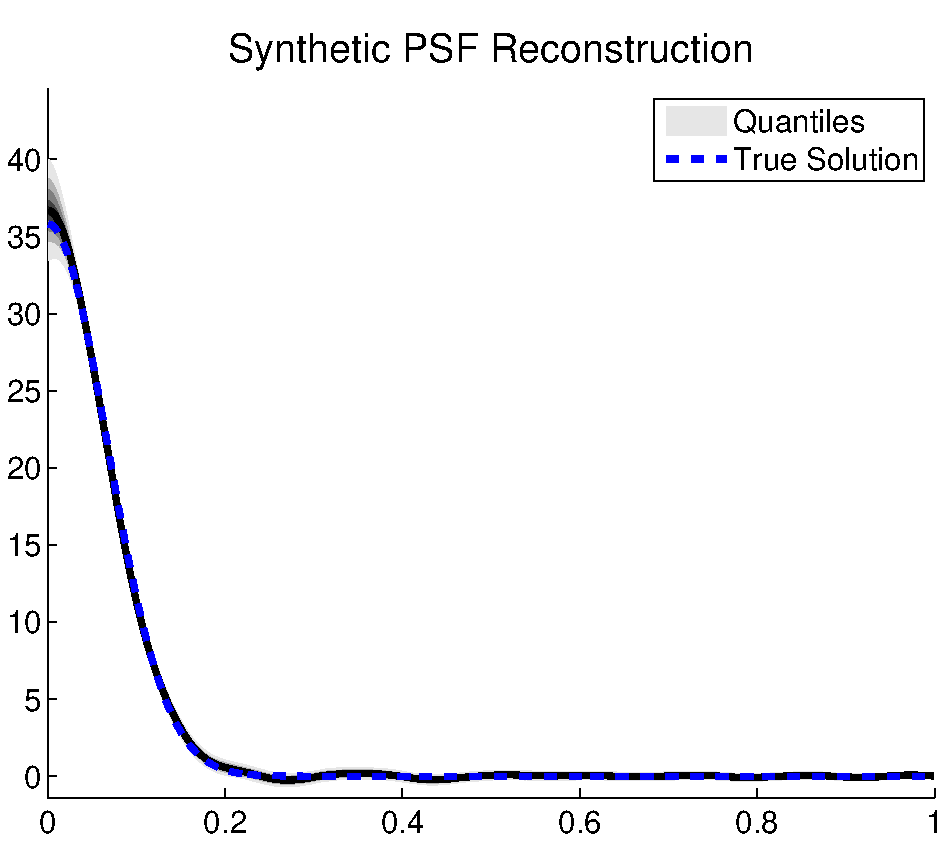
\includegraphics[width=.4\textwidth]{figures/syntheticPSFrecon.pdf}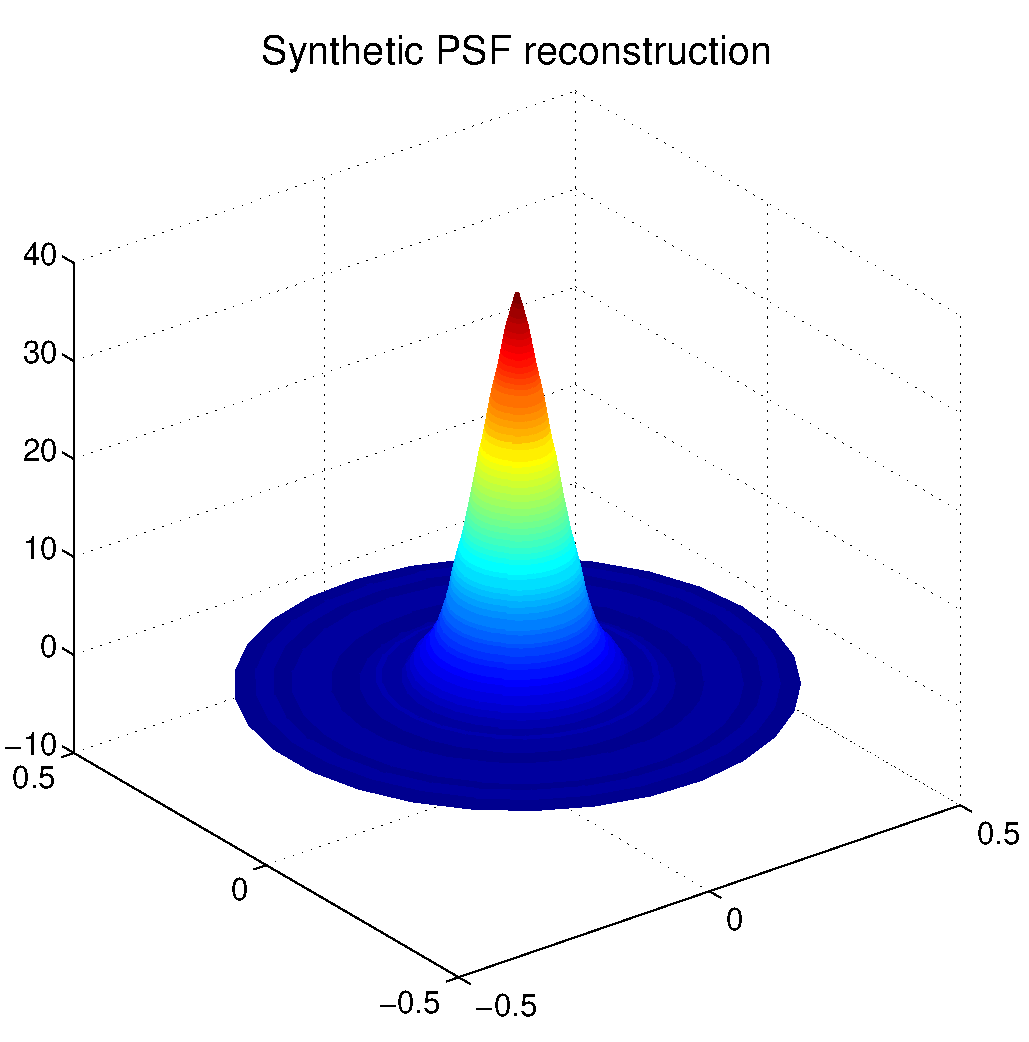
\includegraphics[width=.4\textwidth]{figures/synthetic2dPSFrecon.pdf}
  \caption{The 10\%, 25\%, 50\%, 70\%, and 90\% quantiles of the reconstructed 1D radial representations of the synthetic Gaussian PSF (left) along with the mean 2D reconstruction (right).} \label{fig:syntheticPsfRecon}
  \end{center}
\end{figure}
\begin{figure}[p]
\begin{center}
  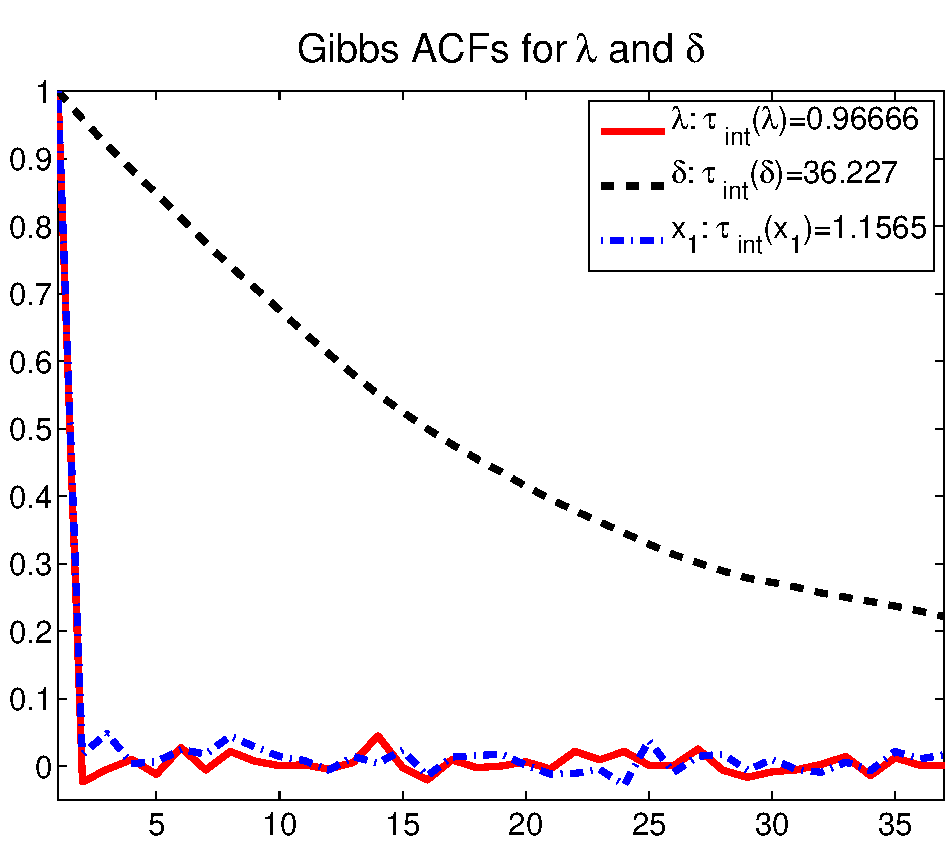
\includegraphics[width=.35\textwidth]{figures/ACFlambdelPSFreconGibbsM1.pdf}  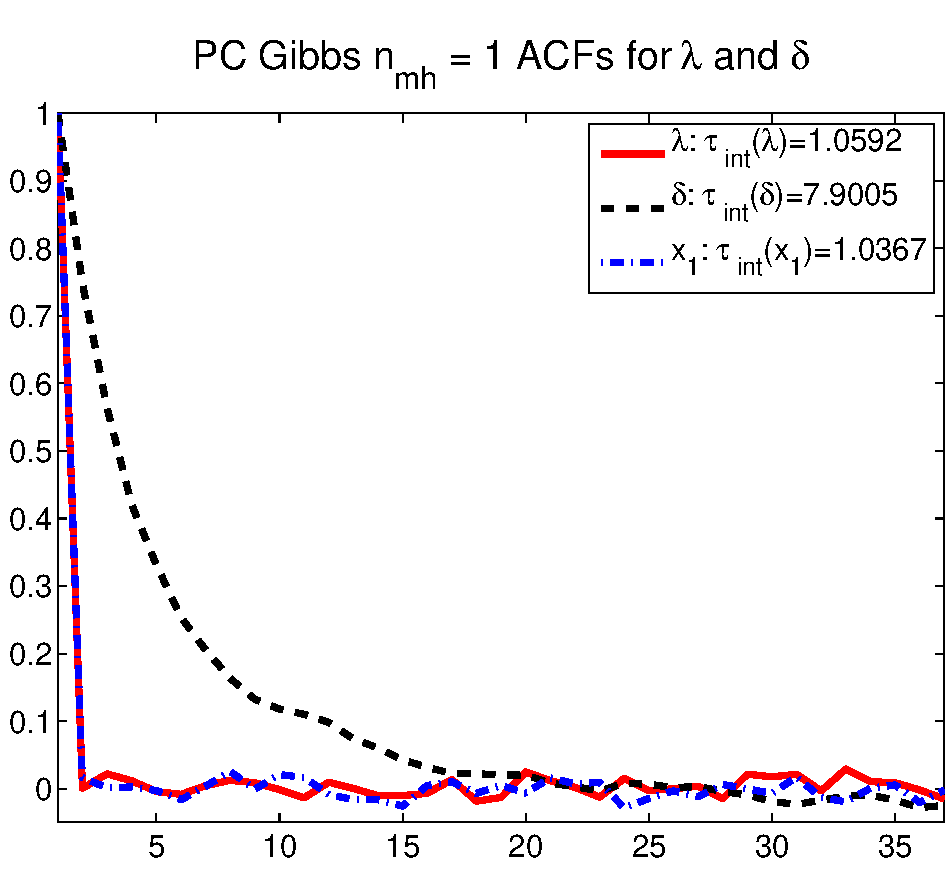
\includegraphics[width=.35\textwidth]{figures/ACFlambdelPSFreconPCGibbsM1.pdf}\\\vspace{2em}
  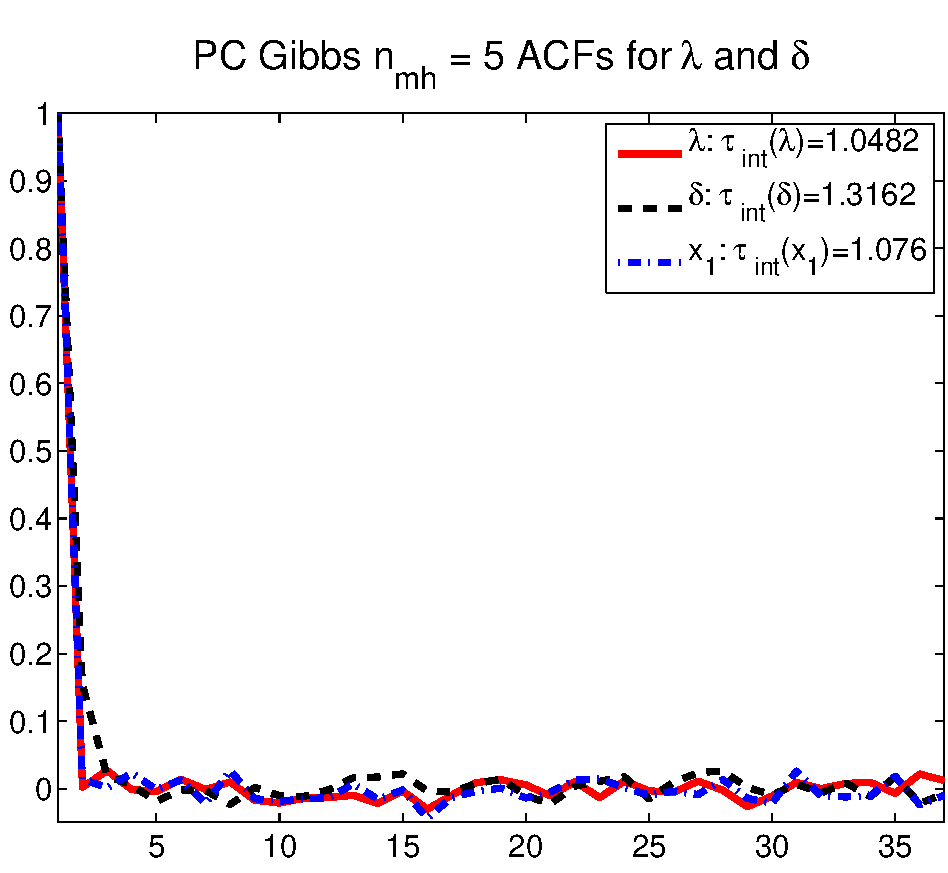
\includegraphics[width=.35\textwidth]{figures/ACFlambdelPSFreconPCGibbsM5.pdf}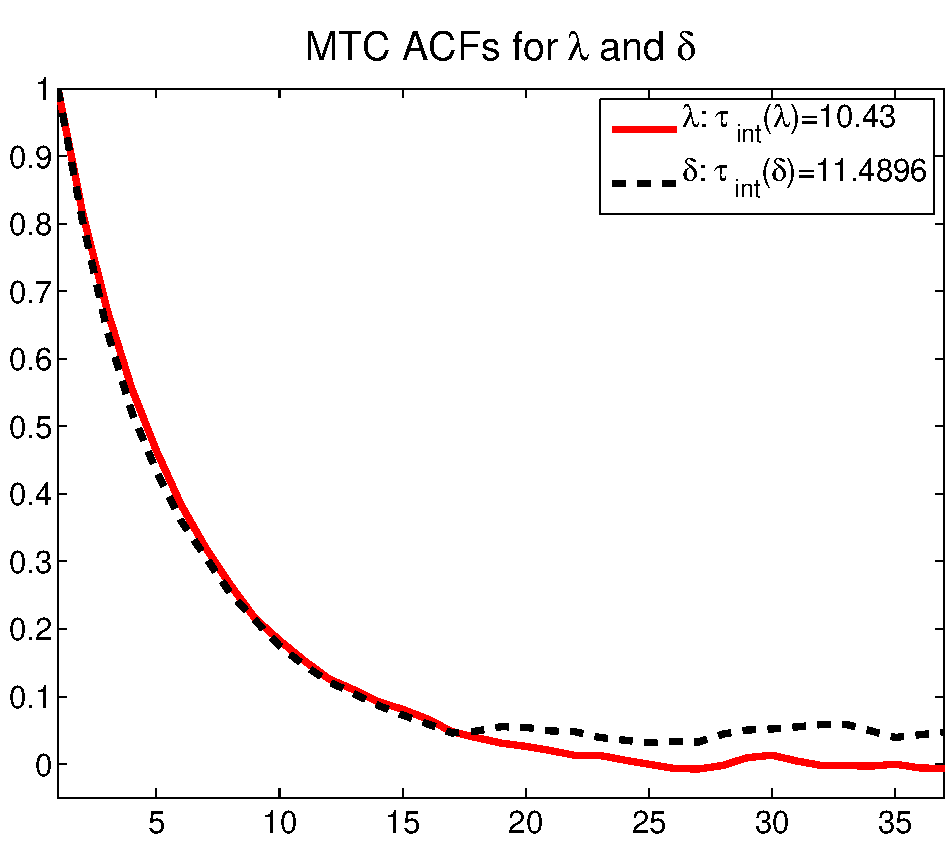
\includegraphics[width=.35\textwidth]{figures/ACFlambdelPSFreconMTC.pdf}
\end{center}
\caption{Autocorrelation plots for PSF reconstruction for synthetic data of the chains $\lambda$, $\delta$ and the central discretization point of $\vect p$: in the upper-left are the ACF for MCMC chains of $\lambda$, $\delta$ and central pixel of the radial profile for the Gibbs sampler; on the upper-right are the plots for the PC Gibbs sampler with 1 inner MH step; on the lower-left are plots for the PC Gibbs sampler with 5 inner MH steps; and in the lower-right are plots for the MTC sampler.} \label{fig:syntheticPsfACF}
\end{figure}

The computed mean of the posterior density is shown in \Cref{fig:syntheticPsfRecon} (right) in 2D, along with quantiles of the radial representations (left). 
The true solution is also shown on the left, showing the accuracy of the reconstruction.  
Note that the most uncertain region of the reconstruction are the initial discretization points corresponding to the height of the PSF, however, the true solution falls within the 90\% quantiles at each point.

The MCMC diagnostics are summarized in \Cref{tab:PSFDeltaChain}. 
With the exception of the $\delta$ chain generated by the Gibbs sampler, each method yields Geweke $p$-values sufficiently large to indicate strong statistical evidence that burn-in has completed. 
The lack of convergence for the Gibbs sampler $\delta$ chain is the likely cause for the mean estimate of $\delta$ being marginally larger than the other three. 
The large autocorrelation in the $\delta$ chain generated by the Gibbs sampler results in an ESS that is significantly lower than the other three algorithms. 
Using \#Chol/ESS as an effeciency measure, we see that PC Gibbs with $n_{mh}=5$ is the most effecient of the four methods.
\begin{table}[h]
\begin{center}
  \begin{tabular}{l|ccccccc}
    \hline
% Jan. 9 values initial delta = 1 and initial lambda = 1
    Algorithm       & $\hat{\lambda}_{\rm MCMC}$& $\hat{\delta}_{\rm MCMC}$  & $\lambda$-$p_{\rm Geweke}$&$\delta$-$p_{\rm Geweke}$& IACT & ESS    & \#Chol/ESS \\
     & $(\times 10^{4})$ & ($\times 10^{-8}$) & & \\
    \hline
	      Gibbs &                 1.102 &                 6.132 &                    0.998 &                    0.850& 36.2 &  138.0 &      72.4 \\
PC Gibbs &                 1.102 &                 5.611 &                    0.992 &                    0.943&  7.9 &  633.0 &      31.6 \\
\hspace{.2in} $n_{mh}= 1$ & & & & & & & \\
PC Gibbs &                 1.102 &                 5.515&                    0.999 &                    0.985&  1.3 & 3799.6 &      15.8 \\
\hspace{.2in} $n_{mh}= 5$ & & & & & & & \\
		MTC &                 1.099 &                 5.419 &                    0.998 &                    0.934& 11.5 &  473.2 &      21.1 \\
    % Dec. 11 values initial delta = norm(B) and initial lambda = 1/var( b(1:10) )
%    Gibbs             &                   0.997 &                    0.850& 46.3 &  107.9 &      92.6 \\
%    PC Gibbs $m_h=1$  &                   0.999 &                    0.955&  5.2 &  954.6 &      21.0 \\
%    PC Gibbs $m_h=5$  &                   0.998 &                    0.981&  1.7 & 2981.8 &      20.1 \\
%    MTC               &                   0.990 &                    0.950& 11.3 &  443.3 &      22.6 \\
    \hline
  \end{tabular}
  \caption{ Statistical diagnostics for the $\lambda$ and $\delta$ chains associated with the synthetic PSF reconstruction problem. The total chain length is $M=10^4$, with a burn-in of $k_{\rm burnin} = 5\times10^3$. The first column are the post-burn-in chain means of $\lambda$ and $\delta$. The maximum IACT of $\lambda$ and $\delta$ are used to calculate IACT and ESS. For MTC algorithm, $\lceil(M-k_{\rm burnin})/\tau_{\rm int}\rceil$ is added to \#Chol to evaluate the efficiency.} \label{tab:PSFDeltaChain}
\end{center}
\end{table}

The chain autocorrelation plots in \Cref{fig:syntheticPsfACF} give additional insights. 
First, for the Gibbs sampler, the autocorrelation of the $\delta$ chain is quite large, and the $\lambda$ chain is approximately uncorrelated, as values in \Cref{tab:PSFDeltaChain} suggested would be the case. 
Note also that sampling jointly in the MTC algorithm degrades the efficiency of $\lambda$. 
Finally, note that we also include autocorrelation plots for the first component, $x_1$, of $\vect p$, in order to show that the $\vect p$ chain is essentially uncorrelated, and hence that the correlation in the MCMC chains generated by Gibbs and PC-Gibbs samplers is driven by the $\delta$ chain. 

\subsection{PSF reconstruction from X-ray Radiographs}\label{subsec:real data}

%We now carry out the analysis outlined above on a synthetic example and on actual data from an X-ray radiographic imaging system at the U.S.~Department of Energy's research complex at the Nevada National Security Site (NNSS) operated by National Security Technologies LLC.

Next we reconstruct the point spread function of a high energy X-ray imaging system at the U.S. Department of Energy's Nevada National Security Site. The real edge data is shown in \Cref{fig:CygnusPsfRecon} (upper left) along with a horizontal cross-section across the edge (upper right). The mean MCMC reconstruction is shown in \Cref{fig:CygnusPsfRecon} (lower left), along with the 10\%, 25\%, 50\%, 70\%, and 90\% quantiles of the chain $\bm{x}^{k}$.
We estimated the PSF at grid points using the chain-wise mean after burn-in, $\hat {\vect p} = \frac 2M \sum_{k=M/2+1}^M {\vect p}^{k}$.
Since the true PSF is unknown, we evaluate the accuracy of the estimation by its discrepancy; i.e. we compared forward mapping of the estimate $\Ab {\hat{\vect p}}$ with the given data $\bm b$.  This is shown in both linear and logarithmic scales in \Cref{fig:CygnusPsfRecon} (lower right). 
In both cases the discrepancy is quite low, except at very low intensities where the data is dominated by the noise, which can be seen in the logarithmic scale.
 %The true solution is not known and is thus not plotted along with the reconstructions.

\begin{figure}[h]
  \begin{center}
  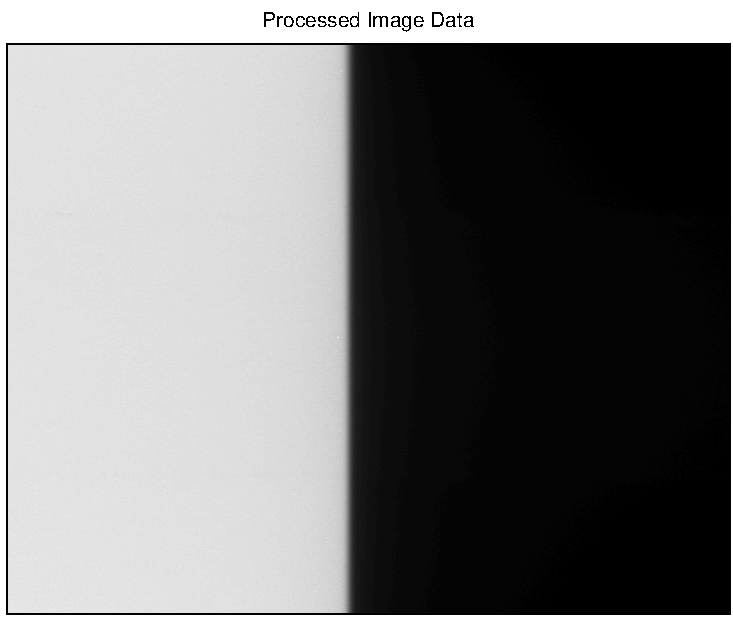
\includegraphics[height=2in]{figures/cygnusImage.pdf}\hspace{2em}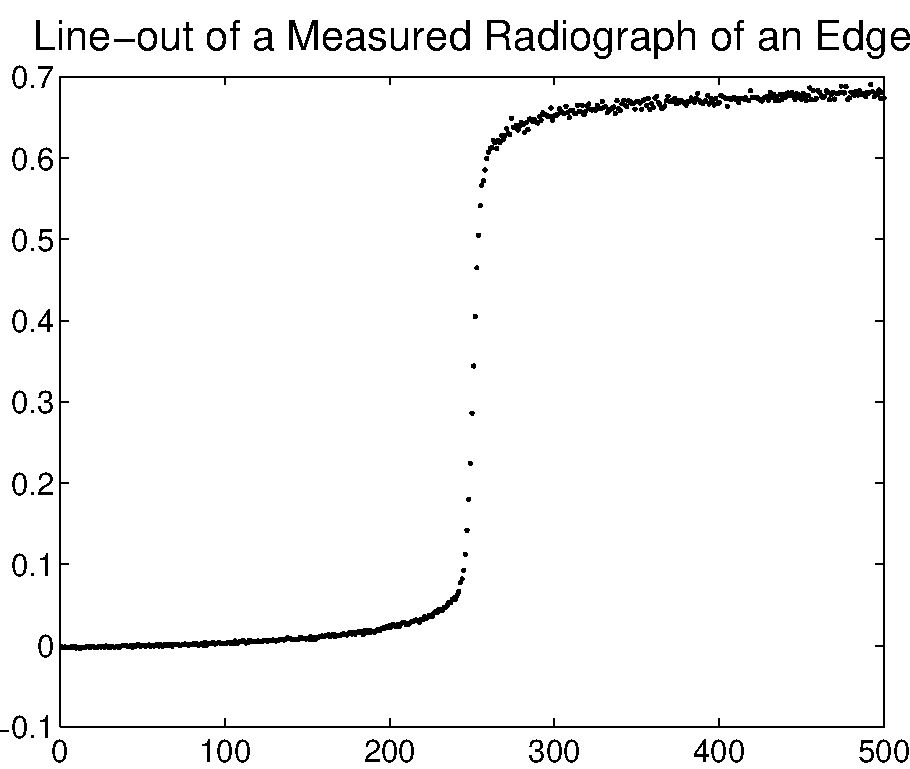
\includegraphics[height=2in]{figures/cygnusLineout.pdf}\\\vspace{2em}
  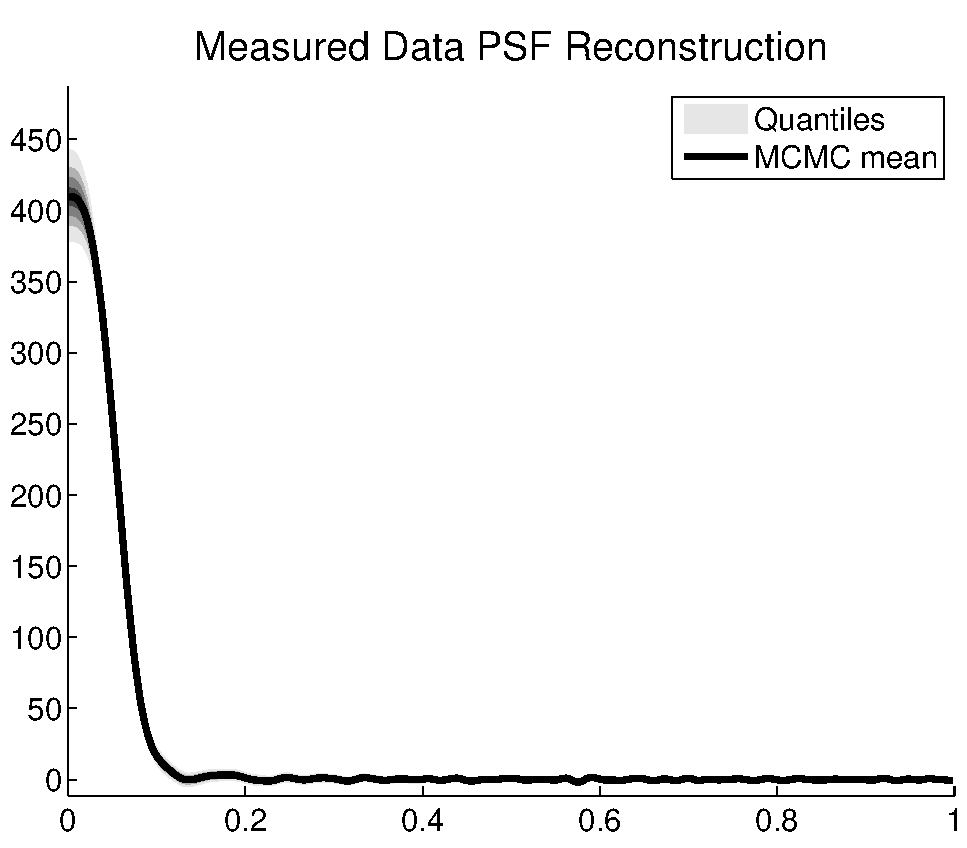
\includegraphics[height=2in]{figures/cygnusPSFrecon.pdf}\hspace{2em}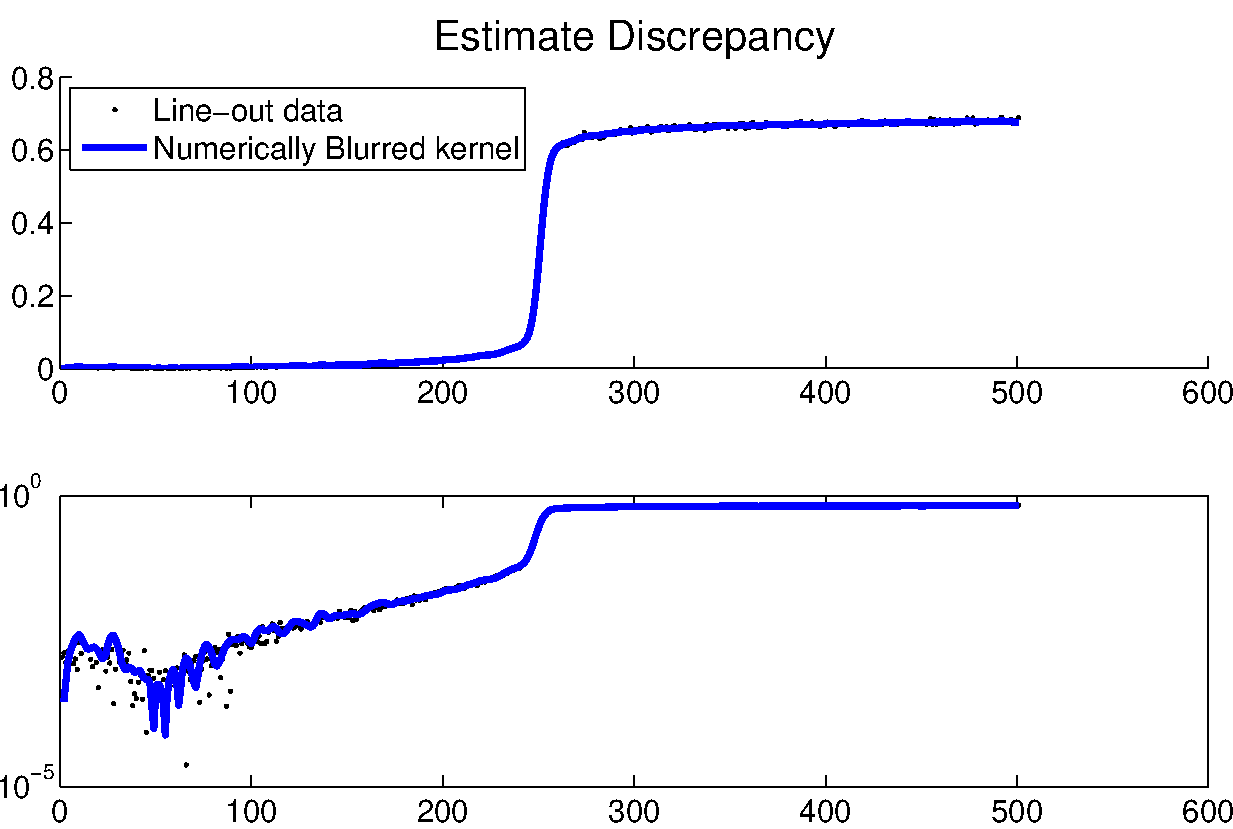
\includegraphics[height=2in]{figures/discrepencyPSF.pdf}
  \caption{
  PSF reconstructions for radiographic data: in the upper left corner are the radiographic image data;
  in the upper right corner is a line-out taken from the image data;
  in the lower left corner are the central 10\%, 25\%, 50\%, 70\%, and 90\% quantiles of the posterior reconstruction of $\bm x$ for each pixel;
  in the lower right corner are plots of the forward mapped discrepancy of the post burn-in chain mean.
  } \label{fig:CygnusPsfRecon}
  \end{center}
\end{figure}

As with the synthetic data, the PC-Gibbs algorithm with $n_{mh}=5$ results in the largest ESS and the most efficient chain (as measured by $\#$Chol/ESS).

\begin{table}[h]
\begin{center}
  \begin{tabular}{l|ccccccc}
    \hline
    Algorithm           & $\hat{\lambda}_{\rm MCMC}$& $\hat{\delta}_{\rm MCMC}$& $\lambda$-$p_{\rm Geweke}$&$\delta$-$p_{\rm Geweke}$& IACT & ESS    & \#Chol/ESS \\
     & $(\times 10^{4})$ & ($\times 10^{-10}$) & & \\
    \hline
	          Gibbs &                 9.146 &               1.245  &                     0.995 &                    0.964& 14.0 &  357.6 &      28.0 \\
PC Gibbs  &                 9.167 &               1.191  &                     0.995 &                    0.998&  8.5 &  587.3 &      34.1 \\
 \hspace{.2in}$n_{mh}=1$ & & & & & & & \\
PC Gibbs &                 9.178 &               1.189  &                     0.994 &                    0.980&  1.5 & 3278.5 &      18.3 \\
\hspace{.2in} $n_{mh}=5$ & & & & & & & \\
		    MTC &                 9.090 &               1.200  &                     0.996 &                    0.969& 12.5 &  432.2 &      23.1 \\
    \hline
  \end{tabular}
  \caption{ Statistical diagnostics for the $\lambda$ and $\delta$ chains associated with the measured data PSF reconstruction problem. The total chain length is $M=10^4$, with a burn-in of $k_{\rm burnin} = 5\times10^3$. The first column are the post-burn-in chain means of $\lambda$ and $\delta$. The maximum IACT of $\lambda$ and $\delta$ are used to calculate IACT and ESS. For MTC algorithm, $\lceil(M-k_{\rm burnin})/\tau_{\rm int}\rceil$ is added to \#Chol to evaluate the efficiency.} \label{tab:CygnusPsfRecon}
\end{center}
\end{table}

\begin{figure}[h]
\begin{center}
  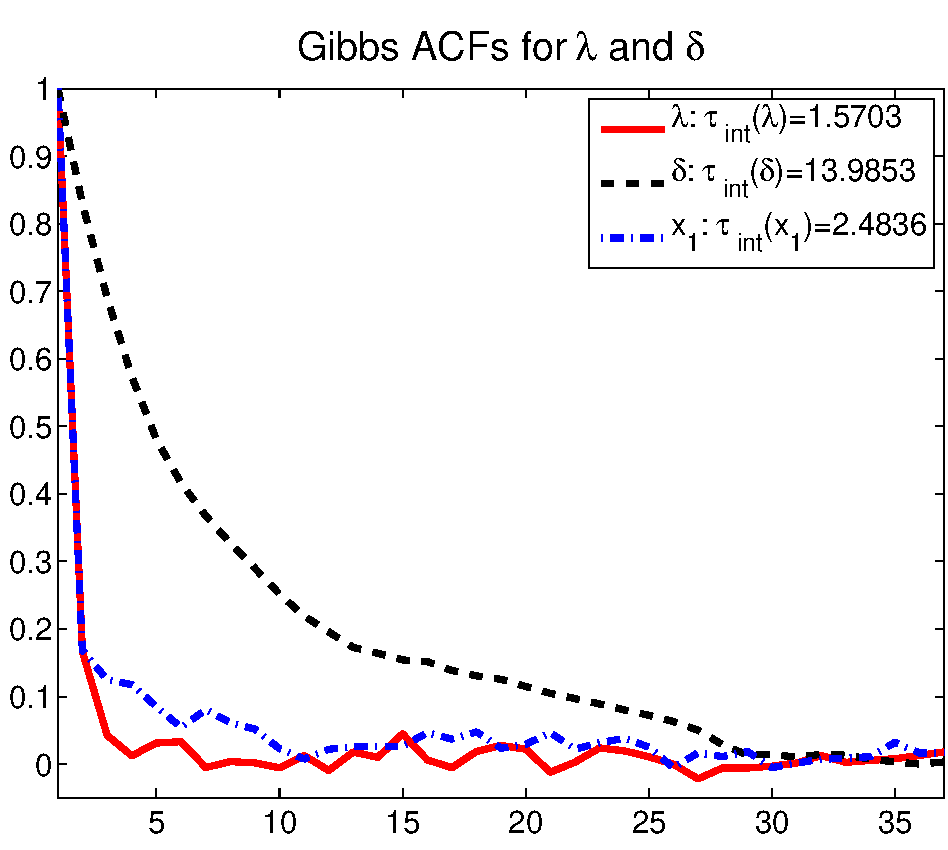
\includegraphics[width=.35\textwidth]{figures/CygnusACFlambdelPSFreconGibbsM1.pdf}  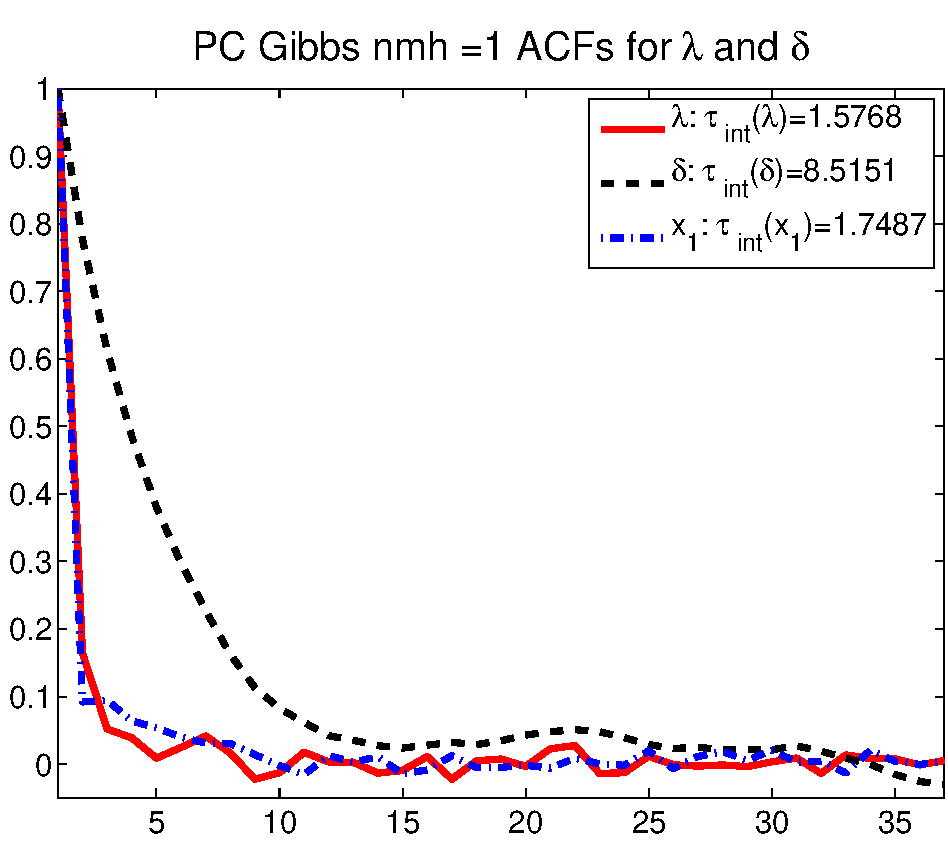
\includegraphics[width=.35\textwidth]{figures/CygnusACFlambdelPSFreconPCGibbsM1.pdf}\\\vspace{2em}
  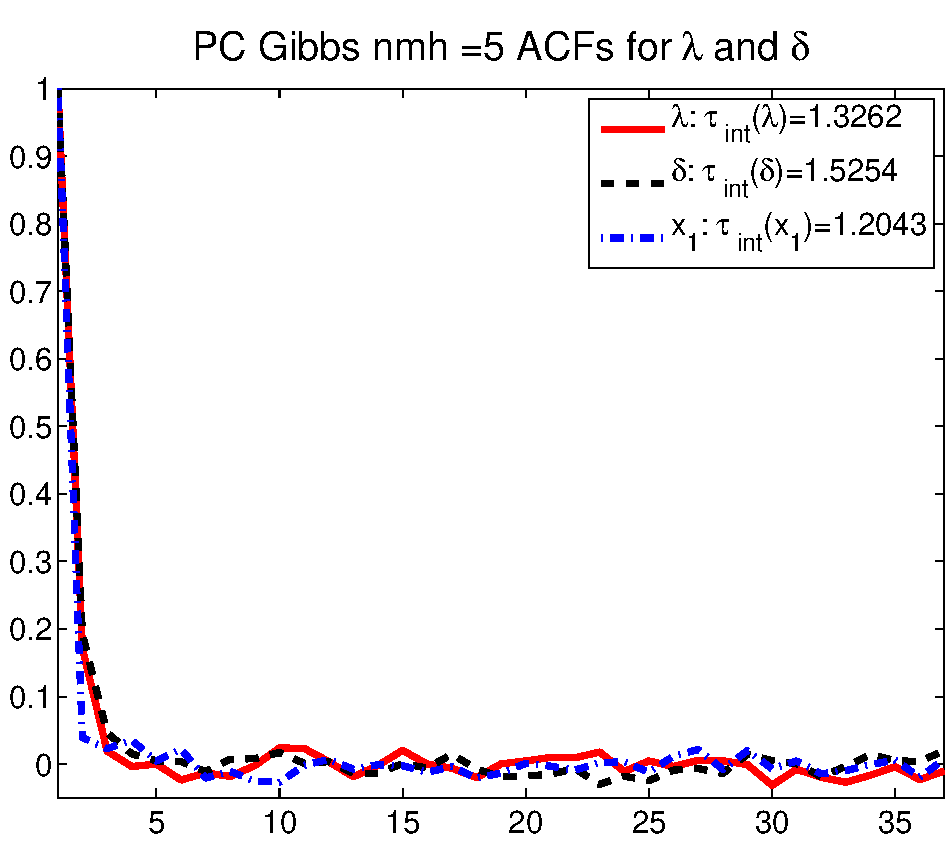
\includegraphics[width=.35\textwidth]{figures/CygnusACFlambdelPSFreconPCGibbsM5.pdf}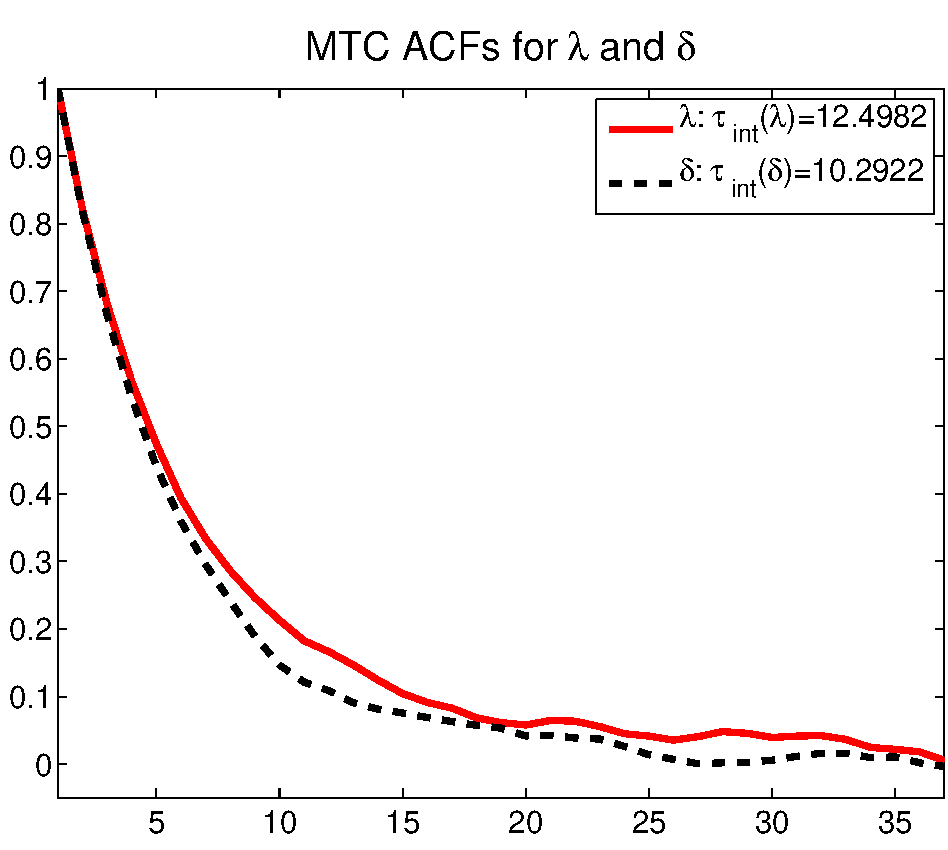
\includegraphics[width=.35\textwidth]{figures/CygnusACFlambdelPSFreconMTC.pdf}
\end{center}
\caption{Autocorrelation plots for PSF reconstruction for the measured data of $\lambda$ and $\delta$ chains: in the upper-left are the ACF for MCMC chains of $\lambda$, $\delta$ and central pixel of the radial profile for the Gibbs sampler; on the upper-right are the plots for the PC Gibbs sampler with 1 inner MH step; on the lower-left are plots for the PC Gibbs sampler with 5 inner MH steps; and in the lower-right are plots for the MTC sampler.} \label{fig:psfACF}
\end{figure}

\subsection{Conclusions} \label{sec:Conclusions}

The synthetic and measured data both exhibit the theoretical degeneracy derived \cite{AgaBarPapStu} for standard Gibbs sampler.
%Specifically, the main theoretical result in \cite{AgaBarPapStu} shows that as the numerical mesh size tends to zero, the autocorrelation of the $\delta$ chain increases, to the extent that in the infinite limit, the MCMC chain will stay fixed on the initial value $\delta_0$. 
%The result is that for problems with a fine mesh, the $\delta$ chain is highly correlated and hence a huge number of samples are needed. 
We've also demonstrated that the issue is alleviated by applying the partially collapsed Gibbs framework to the Gibbs sampler, yielding two related MCMC methods, neither of which have have the $\delta$ chain correlation issues. 
This work provides the first, to our knowledge, successful non-parametric radial PSF reconstruction in X-ray imaging. 
Moreover, the theory for the modeling and algorithms have been rigorously derived from first principles, and may serve as a template for other symmetry based prior regularization schemes.
%Finally, we test our MCMC methods on this inverse problem, using both a synthetic test case and a real data example. 
The results illustrate the effectiveness of the partially collapsed Gibbs approach, and show how a sample-based approach can be used for uncertainty quantification.
\end{chapter}
